\documentclass[12pt,oneside]{article}
\usepackage[russian]{babel}
\usepackage[utf8x]{inputenc}
\usepackage{amsmath}
\usepackage{float}
\usepackage{graphicx}
\usepackage{ textcomp }
\usepackage{xcolor}
\usepackage{hyperref}
\usepackage[colorinlistoftodos]{todonotes}
\usepackage{geometry}
\usepackage{amssymb, gensymb, mathrsfs}
\usepackage{amsthm}
\usepackage{mathtools}
\usepackage{indentfirst}
\usepackage{color}
\usepackage{datetime}
\usepackage{epigraph}
\geometry{a4paper,top=2cm,bottom=2cm,left=2cm,right=2cm}

\newtheorem{statement}{Утверждение}[section]
\theoremstyle{definition}
\newtheorem{definition}{Определение}
\newtheorem{exercise}{Упражнение}
\newtheorem{axiom}{Аксиома}[section]
\newtheorem{exmp}{Пример}[section]
\newtheorem{theorem}{Теорема}[section]
\newtheorem{remark}{Замечание}[section]
\newtheorem{corollary}{Следствие}[section]
\newtheorem{proposition}{Предложение}[section]
\newtheorem{lemma}{Лемма}[section]
\newenvironment{ourproof}[1]{\textit{Доказательство #1.}}{\qed}
\newenvironment{topic}[1]{\textbf{Тема #1.}}{\qed}
\renewcommand{\labelenumii}{\arabic{enumi}.\arabic{enumii}.}


\definecolor{g}{HTML}{006600}
\definecolor{r}{HTML}{FF0000}
\title{Дискретная математика, модуль 1 из 4}
\author{Danił Szubin}
\newcommand{\RomanNumeralCaps}[1]
    {\MakeUppercase{\romannumeral #1}}
\definecolor{linkcolor}{HTML}{799B03} % цвет ссылок
\definecolor{urlcolor}{HTML}{799B03} % цвет гиперссылок
 
\hypersetup{pdfstartview=FitH,  linkcolor=linkcolor,urlcolor=urlcolor,colorlinks=true}



\begin{document}

\maketitle
\footnotesize
\tableofcontents
\normalsize
\newpage
\section{Математическая скоропись. Начала логики.}
\subsection{Высказывания и предикаты}

\begin{definition} \label{statement}
\textbf{Высказывание} \--- осмысленное утверждение, про которое можно однозначно судить: истинно оно или ложно.
\end{definition}

\begin{exmp}

\begin{table}[h!]
\centering
\begin{tabular}{l|r}
Высказывания & Не высказывания \\\hline
$2+1=3$ & $x^2=2$ \\
"Волга впадает в Каспийское море" & "погода хорошая"\\
$1=0$ &  \\
\end{tabular}
\end{table}

Проблема с "погода хорошая"\ в том, что это слишком расплывчатая фраза, нет чётких критериев, чтобы решить, хорошая погода или нет. Проблема с "$x^2=2$"\ в том, что не указано, что такое $x$.
\end{exmp}

\begin{definition} \label{predicat}
\textbf{Предикат (логическая функция)} --- высказывание, зависящее от параметра (т.е. содержащее букву), и указано, что именно можно подставлять вместо буквы. При этом при каждом возможном значении параметра (буквы) должно быть можно сказать: верно это высказывание или нет. 
\end{definition}


\begin{exmp}
Например, ($x^2=2$, где $x$ пробегает множество студентов нашей группы) - это не предикат, потому что не указано, как возводить студента в квадрат и как потом результат этой операции сравнивать с числом, т.е. при подстановке вместо буквы любого из разрешённых значений мы не получаем высказывание (см. определение~\ref{predicat} высказывания выше).

$P(x) = (x^2=1), x=\mathbb{R}$ \--- предикат; логическая функция от одного вещественного переменного $x$

$P(x) = (1=0)$ \--- предикат; логическая функция от нуля переменных, т.е. константа. Причём в данном случае это константа 0, поскольку высказывание 1=0 ложно.
\end{exmp}

\subsection{Кванторы}

\begin{definition}
Кванторы - это значки, которые пишутся перед предикатом. Иногда их можно писать и после предиката, если это не вызывает путаницы при записи нескольких предикатов рядом. Если есть цель полностью избежать путаницы, то надо поставить все кванторы на стандартное для них место --- перед теми предикатами, к которым они относятся. Бывает два квантора: $\forall$ и $\exists$.
\end{definition}

{\bf Квантор всеобщности} $\forall$

$\forall x: P(x)$ \--- для всех/любого/каждого $x$ верно $P(x)$\\

{\bf Квантор существования} $\exists$

$\exists x: P(x)$ \--- существует такой $x$, что верно $P(x)$\\

Обратите внимание: если в предикате каждую из переменных связать квантором, то получится константа.

\subsection{Логические константы}
0 (ложь);
1 (истина);

\subsection{Общеупотребительные логические функции}
\begin{table}[H]
\centering
\begin{tabular}{p{5cm}|c|p{5cm}|c}
Название & Значок & Прочтение & Таблица истинности \\\hline
Конъюнкция & $\wedge$, $\&$, & $x\wedge y$, "x и y" &
    \begin{tabular}{c|c|c|c|c}
    \centering
    $x$&0&0&1&1 \\\hline
    $y$&0&1&0&1 \\ \hline
    $x\wedge y$&0&0&0&1 \\
    \end{tabular}
                                                        \\\hline
Дизъюнкция (Неисключающее "или") &$\vee$, or &$x\vee y$, "x или y" &
    \begin{tabular}{c|c|c|c|c}
    \centering
    $x\vee y$&0&1&1&1 \\
    \end{tabular}
                                                        \\\hline
Исключающее "или" & $\oplus$, xor &$x\oplus y$, "x либо y" &
    \begin{tabular}{c|c|c|c|c}
    \centering
    $x\oplus y$&0&1&1&0 \\
    \end{tabular}
                                                        \\\hline
Импликация & $\to$ & $x\to y$, "из x следует y"  &
    \begin{tabular}{c|c|c|c|c}
    \centering
    $x\to y$&1&1&0&1 \\
    \end{tabular}
                                                        \\\hline
Эквивалентность & $\leftrightarrow$, $\Leftrightarrow$ & $x\leftrightarrow y$, "x логически эвивалентноно y" &
    \begin{tabular}{c|c|c|c|c}
    \centering
    $x\leftrightarrow y$&1&0&0&1 \\
    \end{tabular}    
                                                        \\\hline
Отрицание & $\neg$, $\bar x$& $\bar x$, "не верно, что x" &
    \begin{tabular}{c|c|c}
    \centering
    $x$&0&1 \\\hline
    $\bar x$&1&0 \\
    \end{tabular}
                                                        \\\hline

\end{tabular}
\end{table}

\begin{remark}
Запись $a\longrightarrow b$ означает <<из $a$ следует $b$>>. Эта связь между $a$ и $b$ может быть равносильно выражена так:
\\$a$ -- достаточное условие для $b$;
\\$b$ -- необходимое условие для $a$;
\end{remark}

\section{Множества и операции с ними}
{\it Неформальное описание: } \textbf{Множество} \--- набор, неупорядоченный список, куча, семейство каких-либо объектов, отличимых друг от друга и от всех остальных объектов материального и интеллектуального мира, называемых \textbf{элементами}.
\begin{remark}[]

\begin{enumerate}

    \item В множестве все элементы разные, не повторяются.
    \item Множество --- одно из основных понятий математики. При современном подходе каждый новый вводимый в рассмотрение объект определяется как некоторое множество.
    \item Подходы к теории множеств
        \begin{itemize}
            \item наивный (нет аксиом, интуитивное понимание множества через описание)
            \item аксиоматический
        \end{itemize}
\end{enumerate}
\end{remark}

{\it Неформальное описание: } \textbf{Функция (в широком смысле)}, определённая на множестве $A$ и принимающая значения в множестве $B$ --- это правило, способ, по которому каждому элементу $x$ множества $A$ сопоставлен ровно один элемент $f(x)$ множества $B$.
$f: A\longrightarrow B $ \--- функция $f$ отображает $A$ в $B$ \newline
$y=f(x)$ \--- значение функции $f$ на элементе $x$ равно элементу $y$ \newline
$f: x\mapsto f(x)$ \--- $f$ переводит элемент $x$ в элемент $f(x)$ \newline
$f = [x\mapsto f(x)]$ \--- $f$ \--- это та функция, которая $x$ переводит в $f(x)$ \newline 

{\it Неформальное описание: } \textbf{Функция (в узком смысле)} \--- функция в широком смысле, заданная на числовом множестве и принимающая числовые значения, т.е. $A$ и $B$ \--- некоторые множества чисел.
Если $f: A\longrightarrow B$, то $A$ называется областью определения функции ($D(f), D_{f}, Dom(f)$, а $B$ \--- множеством значений. (Не путать с множеством всех принимаемых значений)\newline
\begin{exmp}
$A=B=\mathbb{R}, f(x)=sin(x)$

$D(f) = A = \mathbb{R}$ \--- область определения

$B = \mathbb{R}$ \--- множество значений

$E(f)=[-1;1]$ \--- множество всех принимаетмых значений
\end{exmp}

$x\in A$ \--- "$x$ лежит в $A$"

$A\ni x$ \--- "$A$ содержит $x$"

Если из $x\in A$ следует $x\in B$, то говорят, что $A$ является \textbf{подмножеством} в множестве $B$, это записывается как
$A\subset B$ и 
$B\supset A$. При этом $B$ называется \textbf{надмножеством} для $A$.\newline \newline
$\varnothing $ \ \ \--- \textbf{пустое множество}, т.е. множество, в котором нет элементов


\subsection{Способы задания множеств}
\begin{enumerate}
    \item Явное перечисление (годится для небольших множеств)\newline
        $A = \{1, 2, a, *\}$\ \ \---"множество $A$ содержит элементы $1, 2, a, *$ и не содержит других элементов"
        
    \item Задание с помощью свойства или правила (предиката)\newline
        $A=\{x: P(x)\}$\ \ \--- "$A$ состоит из тех $x$, для которых верно $P(x)$".  Внимание! Должно быть явно указано, что можно подставлять в качестве $x$. Иначе могут возникнуть парадоксы, об этом будет сказано в конце курса. \newline
        $\{x: x^2\leq 4, x\in \mathbb{R} \} = [-2; 2]$
    \item Множество можно выразить через уже известные множества и операции над множествами.
    \item Множество можно задать с помощью характеристической функции
\end{enumerate}
\begin{remark}
    Будем считать, что все рассматриваемые нами множества содержатся в каком-то одном большом множестве $U$. То есть мы не рассматриваем сколь угодно большие множества, а оперируем только подмножествами множества $U$.
    \end{remark}
\begin{definition} \label{Char_f}
\textbf{Характеристической функцией} $\chi_{A}$ множества $A (A\subset U)$ называется функция, принимающая значение $1$ на элементах множества $A$ и значение $0$ на остальных элементах множества $U$.
\end{definition}
$\chi_{A}(x) =
        \begin{cases} 
        1, & x\in A \\
        0, & x\not\in A \\
        \end{cases} $
\newline \newline
$\chi_{A}: U \longrightarrow \{0, 1\} $
\newline
\subsection{Операции над множествами}
\begin{table}[H]
    \centering
    \begin{tabular}{p{0.1\linewidth}| p{0.1\linewidth}| p{0.25\linewidth}| p{0.2\linewidth}| p{0.2\linewidth}}
         Обозна-чение & Название & Определение & Диаграмма Эйлера &  Характеристическая функция \\\hline
         
         $A\cap B$ &
         пересече-ние & 
         $x\in A\cap B \leftrightarrow \newline \leftrightarrow (x\in A)\wedge (x\in B)$ &
         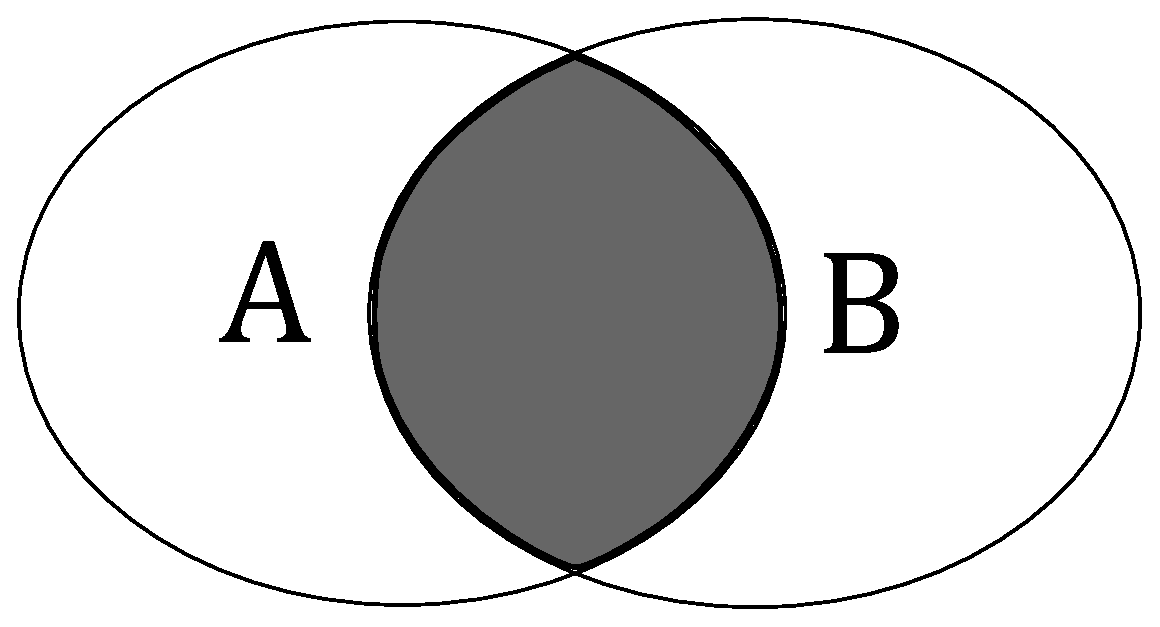
\includegraphics[width=0.2\textwidth]{intersect.eps}
         &
         $\chi_{A\cap B}=\chi_{A}(x)\chi_{B}(x)$ \\\hline
         
         $A\cup B$& объеди-нение\newline $A$ и $B$ &
         $x\in A\cup B \leftrightarrow \newline \leftrightarrow (x\in A)\vee (x\in B)$ &
         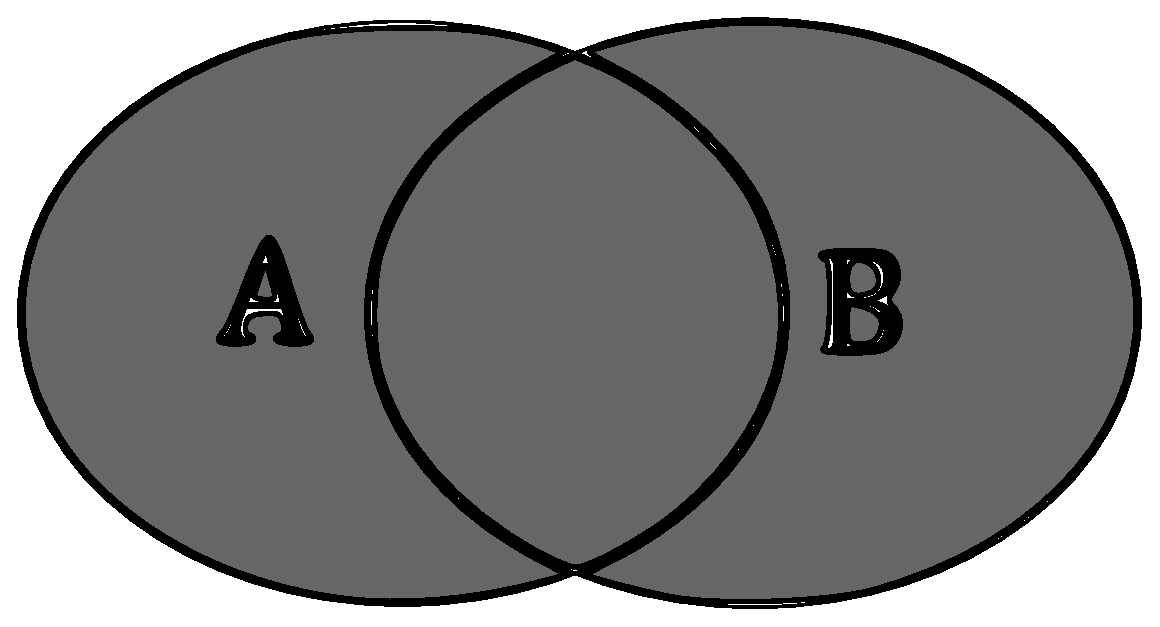
\includegraphics[width=0.2\textwidth]{union.eps}
         &
         $\chi_{A\cup B}=\chi_{A}(x)+\chi_{B}(x)-\chi_{A}(x)\chi_{B}(x)$ \\\hline
         
         $A\setminus B$ & 
         $A$ без $B$ & 
         $x\in A\setminus B \leftrightarrow \newline \leftrightarrow (x\in A)\wedge (x\notin B)$& 
         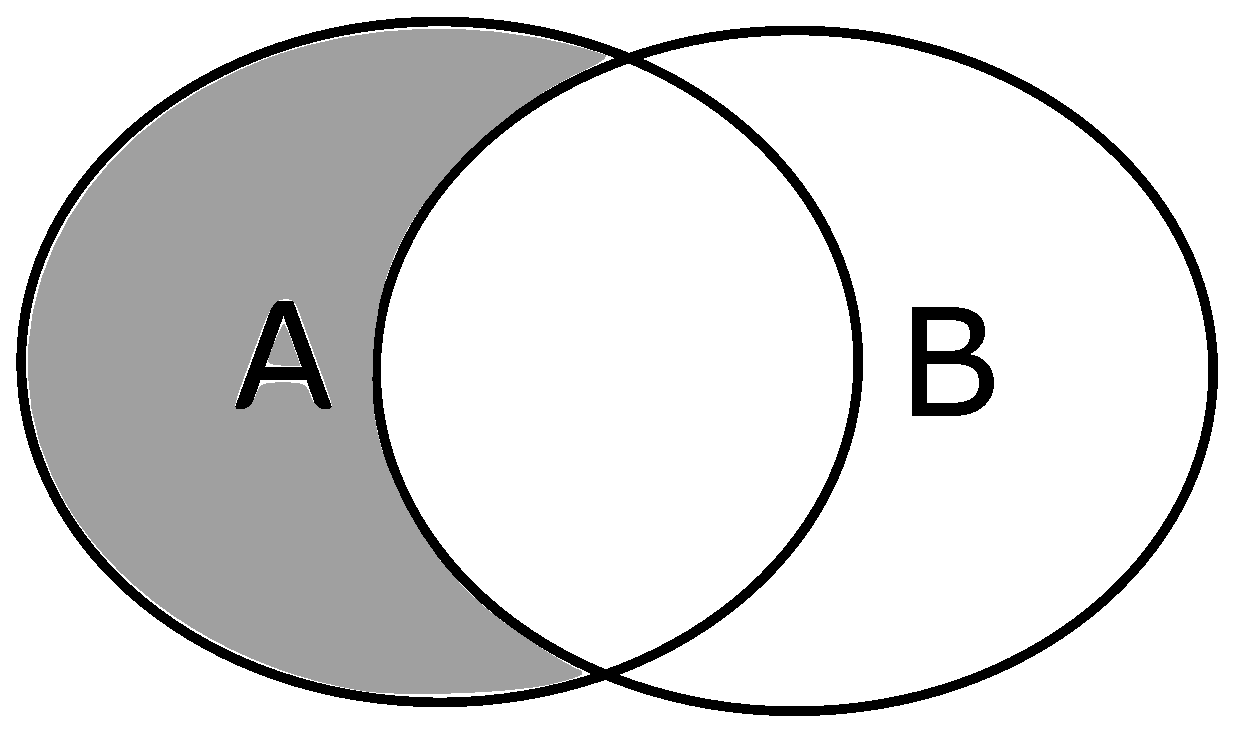
\includegraphics[width=0.2\textwidth]{setminus.eps}
         & 
         $\chi_{A\setminus B}(x)=\chi_{A}(x)--\chi_{A}(x)\chi_{B}(x)$\\\hline
         
         $A\bigtriangleup B$ &
         Симмет-рическая разность $A$ и $B$ &
         $x\in A\bigtriangleup B \leftrightarrow \newline \leftrightarrow (x\in A)\oplus(x\in B)$ 
         &
         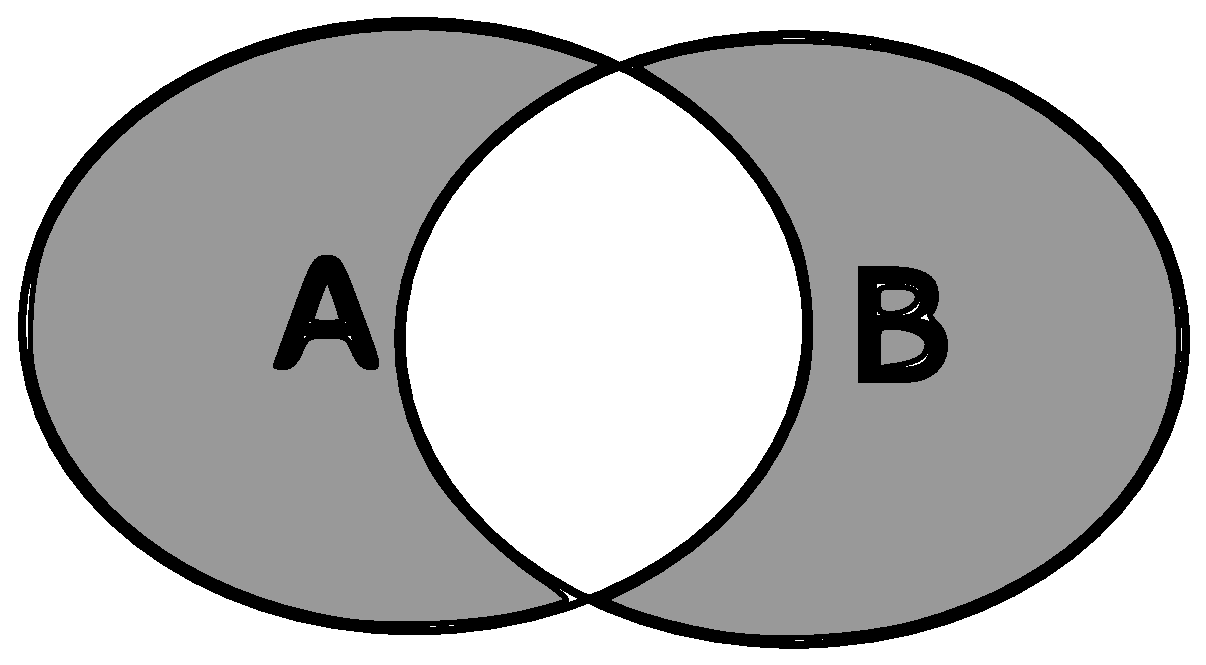
\includegraphics[width=0.2\textwidth]{simdiff.eps}
         & $\chi_{A\bigtriangleup B}(x)= \chi_{A}(x) + \chi_{B}(x) - 2\chi_{A}(x)\chi_{B}(x)$ \\\hline
         
         $\neg A, A^C$ &
         Дополне-ние (comple-mentary) мн-а $A$ &
         $x\in \neg A \leftrightarrow$ \newline $\leftrightarrow x\not \in A$ &
         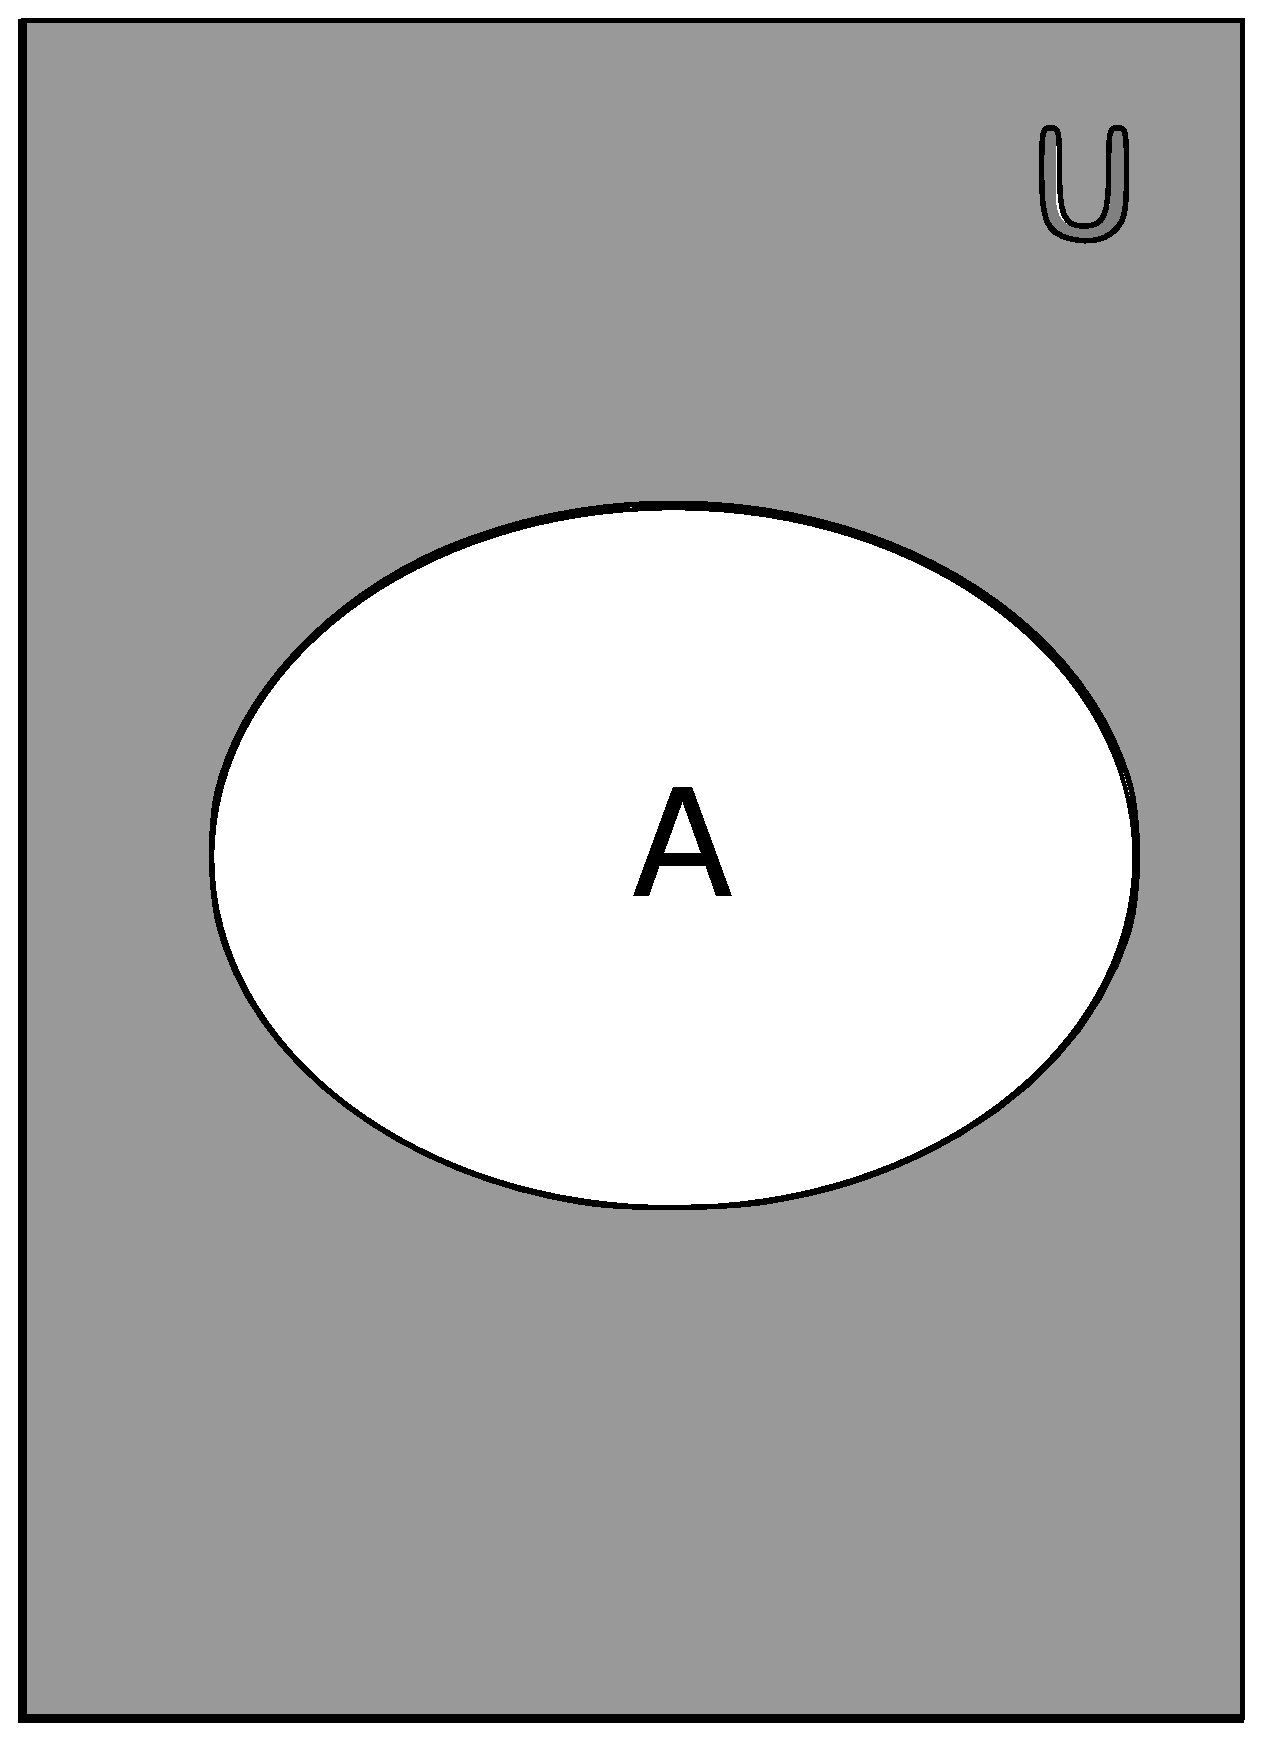
\includegraphics[width=0.2\textwidth]{dop.eps}
         &
         $\chi_{\neg A}(x)= 1 - \chi_{A}(x)$
    \end{tabular}
    \label{tab:my_label}
\end{table}

\subsection{Круги Эйлера, диаграммы Венна}
1)Как обойтись совсем без картинок при сравнении множеств?
\newline
\begin{tabular}{c|c|c|c|c|c|c}
         & $A$ & $\overline{A}$ & $B$ & $\overline{B}$ & $C$ & $\overline{C}$ \\\hline
         $A\setminus B$ &1&0&0&1&1&1\\\hline
         $(A\setminus B)\cap C$&1&0&0&1&1&0\\
\end{tabular}

2)Как нарисовать картинку для $n\geqslant 3$ множеств? 

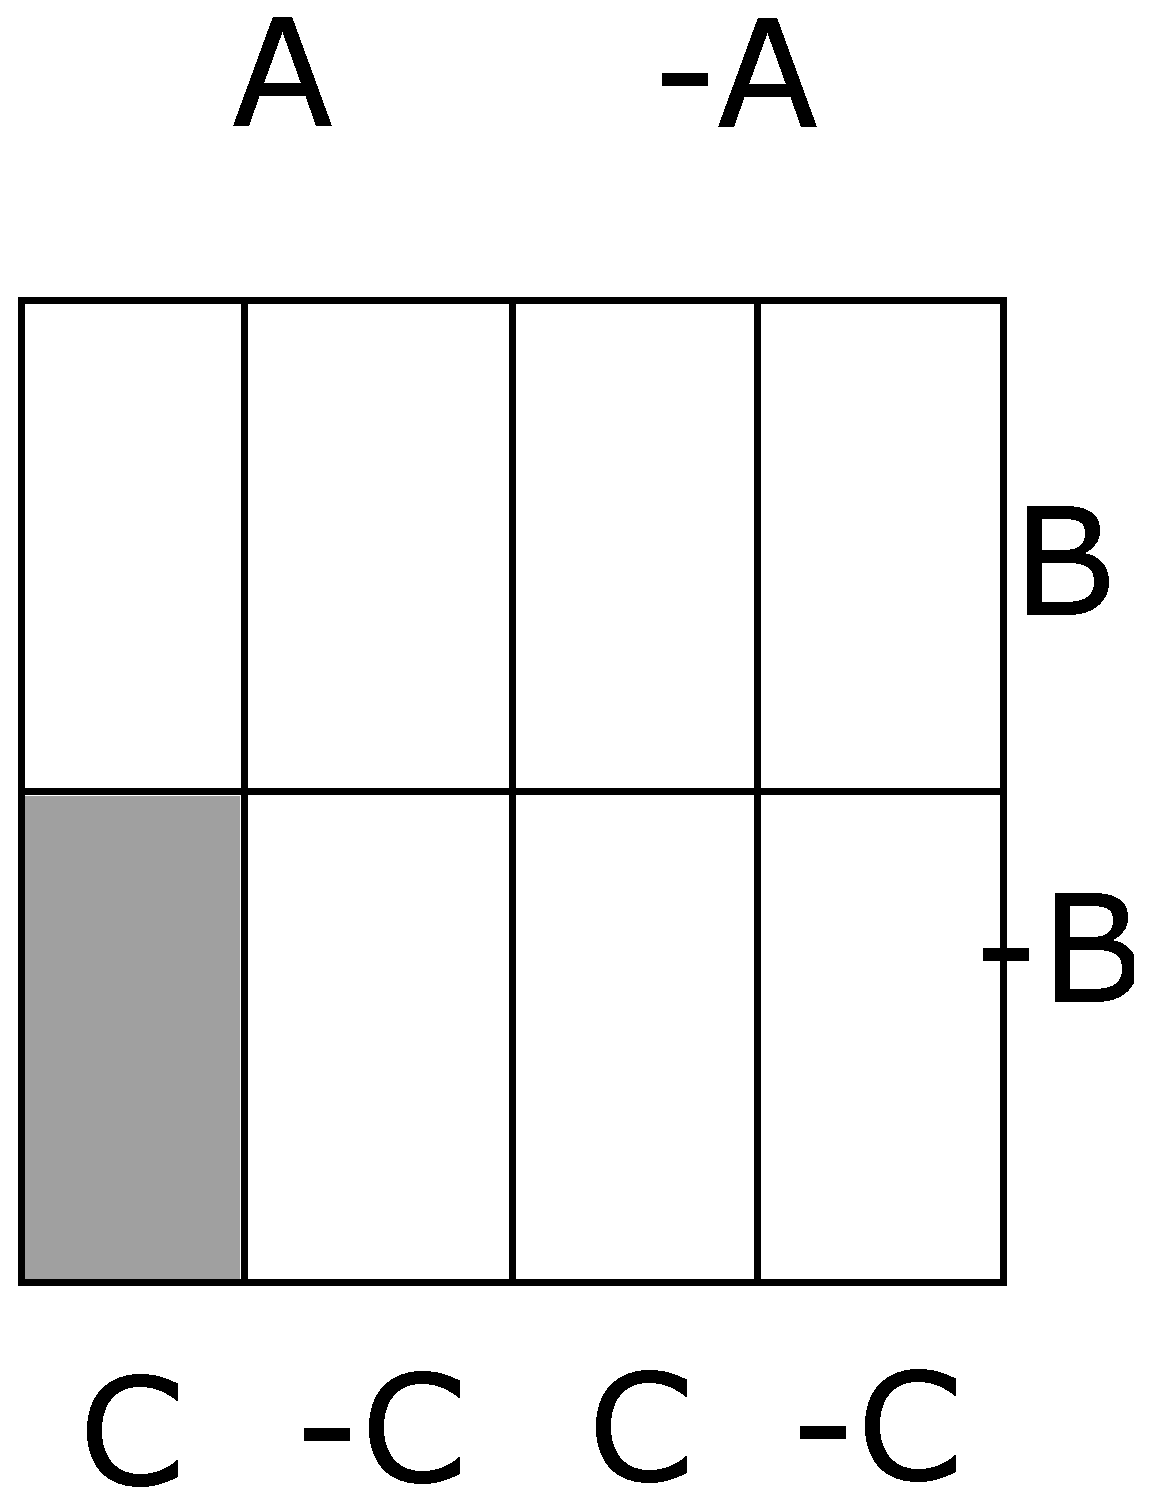
\includegraphics[width=0.2\textwidth]{ris.eps}

\begin{definition}
Если $A$ --- множество, то символами $2^A$ и $\mathcal{P}(A)$ и $\mathscr{P}(A)$ обозначается множество всех подмножеств множества $A$, т.е. $2^A = \mathcal{P}(A) = \mathscr{P}(A) = \{B: B\subset A\}$.
\end{definition}

\begin{remark}
Почему используется обозначение $2^A$? Если $A$ --- конечно, то в множестве $2^A$ ровно $2^n$ элементов. Обозначая количество элементов в конечном множестве $M$ символом $|M|$, получаем равенство $\left|2^A\right|=2^{|A|}$.
\end{remark}

\begin{theorem}\label{teorem_2A}
Если в множестве $A$ ровно $n$ элементов, то у множества $A$ ровно $2^n$ подмножеств.
 
\begin{proof}{}
{\it 1 способ: } 
$A = \{a_{1}, ..., a_{n}\}$. Тогда каждое множество $B\subset A$ однозначно задаётся своей характеристической функцией
$\chi_{B}: A \leftarrow \{0, 1\}$.

$\chi_{B}(a_{1}), ..., \chi_{B}(a_{n})$ --- строка из $0$ и $1$ длины $n$. Сколько таких строк, столько и возможных характеристических функций, столько и существует подмножеств у множества $A$. Всего строк $2^n$, так как эти строки задают двоичное разложение целых чисел от 0 (строка из всех нулей) до $2^n-1$ (строка из всех единиц).
\newline
{\it 2 способ: }
\newline
\textbf{База: } $n=0, A=\varnothing$, $2^A=\{\varnothing\}$ --- множество из одного элемента, этот элемент --- $\varnothing$.
\newline
$2^n = 2^0 = 1$ - верно
\newline
\textbf{Предположение: } У множества из $n$ элементов ровно $2^n$ подмножеств.
\newline
\textbf{Шаг: } Пусть в множестве $B$ ровно $n+1$ элементов. Докажем, что у $B$ ровно  $2^{n+1}$ подмножеств.
\newline
т. к. $B\neq \varnothing$, то выберем любой элемент $b\in B$. Тогда все подмножества множества $B$ распадаются на 2 типа:
\newline
1. Не содержащие $b$, т. е. подмножества множества
$B\setminus\{b\}$, в котором $n$ ($2^n$ подмножеств).
2. Содержат $b$, т.е. $(\{b\}\cup C, C\subset B\setminus\{b\}$. Поэтому их тоже $2^n$ штук.
\newline
Все подмножества множества $B$: 
\newline
$2^n + 2^n = 2*2^n = 2^{n+1})$
\end{proof}
\end{theorem} 

\begin{definition}Если $A\cap B=\varnothing$, то говорят, что множества $A$ и $B$ дизъюнктные. Выражение $A\sqcup B$ называют дизъюнктной суммой (дизъюнктным объединением) множеств $A$  и $B$, то есть


$C = A\sqcup B \Longleftrightarrow $
$\begin{cases} 
        C = A\cup B\\
        A\cap B \neq \varnothing\\
\end{cases}$
\end{definition}


\subsection{Формула включений-исключений}
{\it Обозначение: } Если $A$ "--- конечное множество, то символы $|A|$, $\#A$, $Card(A)$ обозначают количество элементов в множестве $A$.
\newline
{\it Пример: } $|\{1, a, *\}| = \#\{1, a1 *\} = Card(\{1, a, *\}) = 3$
\newline
$|\varnothing | = 0$
\newline
Формула включений-исключений для двух множеств

$|A\cup B = |A| + |B| - |A\cap B|$
\newline

Формула включений-исключений для трёх множеств

$|A\cup B\cup C| = |A| + |B| + |C| - |A\cap B| - |A\cap C| - |B\cap C| + |A\cap B\cap C|$

Формулу включений-исключений можно записать для любого конечного числа множеств, подробнее см. Википедию.

\section{Бинарные отношения}
\epigraph{Общество - это множество людей и отношений между ними.}{И. Ремизов 2006г.}

\begin{definition}
Если $x\neq y$, то множество $\{x,\ y\} $ называется \textbf{неупорядоченной парой} $x$ и $y$.
\end{definition}

\begin{remark}
Все множества первоначально предполагаются не имеющими никакой внутренней структуры: их нельзя складывать, сравнивать, какой из них больше, и так далее. Сложение, порядок и так далее должны быть специально определены, поэтому между множествами $\{x,\ y\}$ и $\{y,\ x\}$ нет разницы (то есть $\{x,\ y\} = \{y,\ x\}$), так как обе эти записи говорят лишь, какие элементы входят в множество. У множеств $\{x,\ y\}$ и $\{y,\ x\}$ одни и те же элементы, поэтому множества $\{x,\ y\}$ и $\{y,\ x\}$ равны. Если $x=y$, то неупорядоченная пара $\{x,\ y\}$ содержит по факту только один элемент (так как $x$ и $y$ --- один и тот же элемент), поэтому $\{x,\ x\} = \{x\}$.
\end{remark}

\begin{definition}
\textbf{Упорядоченной парой} называется множество $\langle x,\ y\rangle = \{ \{x,\ y\},\ \{x\} \} $. Элемент $x$ здесь называется первым элементом пары, а $y$ --- вторым.
\end{definition}

\begin{remark}
Если $x\neq y$, то $ \langle x,\ y\rangle = \{ \{x,\ y\},\ \{x\} \} \neq \{ \{x,\ y\},\ \{y\} \} = \langle y,\ x\rangle$.
\end{remark}

\begin{definition}\label{dec_mult}
Пусть $A$ и $B$ - множества. \textbf{Декартовым произведением} $A$ и $B$ называют множество всех упорядоченных пар, в которых первый элемент из $A$, а второй "--- из $B$.
$\langle a, b \rangle$ - упорядоченная пара
$A\times B = \{\langle a, b\rangle : a\in A, b\in B\}$
\end{definition}

\begin{definition}\label{bin_relation}
\textbf{Бинарным отношением} на $A\times B$ (другой термин "--- \textbf{соотношение} из $A$ в $B$) называется подмножество в $A\times B$.
\end{definition}

$R\subset A\times B,\ \ R $ "--- соотношение из $A$ в $B$.

$R$ "--- те пары $\langle a, b\rangle$, которые состоят в отношении $R$

{\it Обозначение: } $\langle a, b\rangle \in R \Leftrightarrow aRb$

Графиком отношения $R$ называют отношение $R$



\subsection{Свойства бинарных отношений}

\begin{definition}
Отношение $R$ на множестве $A$ называется 
\begin{itemize}
    \item \textbf{рефлексивным}, если $aRa \forall a\in A$. Геометрический смысл: диагональ принадлежит бинарному отношению.
    \item \textbf{антирефлексивным}, если $a\overline{R}a \forall a\in A$. Геометрический смысл: диагональ не пересекается с графиком отношения.
    \item \textbf{симметричным}, если $xRy \Longleftrightarrow yRx \quad \forall x\in A,\quad y\in A$. Геометрический смысл: график симметричен относительно диагонали.
    \item \textbf{антисимметричным}, если $(xRy \wedge yRx) \Longrightarrow y=x$. Геометрический смысл: симметричные относительно диагонали точки графика могут лежать только на диагонали.
    \item \textbf{связным}, если $xRy \vee yRx\quad \forall x\in A,\quad y\in A$. 
    \item \textbf{транзитивным}, если $xRy\wedge yRz \Longrightarrow xRz\quad \forall x\in A,\quad y\in A,\quad z\in A$
\end{itemize}

\begin{definition}
Отножение $R$ на множестве $A$ называется \textbf{отношением предпочтения}, если оно связно и транзитивно. Пример: пусть $A$ --- непустое множество, и дана функция (называемая функцией полезности) $f\colon A\to\mathbb{R}$, тогда можно положить $xRy\iff f(x)\leq f(y)$. Проверьте, что $R$ --- отношение предпочтения.
\end{definition}

\begin{remark}
Оказывается, что не каждое отношение предпочтения можно задать с помощью функции полезности.
\end{remark}

\end{definition}


\subsection{Отношение эквивалентности}
\begin{definition}
R называется \textbf{отношением эквивалентности} если и только если оно рефлексивно, симметрично и транзититвно.
\end{definition}
\begin{definition}
\textbf{Разбиением множества} $A$ на $A_{\omega} \  \omega \in \Omega$ называется представление $A$ в виде дизъюнктной суммы множеств $A_\omega$, то есть $A = \displaystyle\bigsqcup_{\omega \in \Omega} A_{\omega} $, по использованному обозначению см. раздел \ref{indexing}.
\end{definition}
%НАЧИНАЮТСЯ ТЕОРЕМЫ И ДОКАЗАТЕЛЬСТВА
\begin{definition}
$M$ --- множество и R --- отношение эквивалентности на $M$. \textbf{Классом эквивалентности элемента} $x\in M$ называется множество $K_{x} = [x] = \{y\in M\ |\ x
Ry\}$
\end{definition}

\begin{theorem} \label{eq_t}
$[x]\cap [y]\neq \varnothing \Longrightarrow [x]=[y]$
\newline
\begin{ourproof}{}

Если $[x]\cap [y]\neq \varnothing$, то $\exists z\in M: (z\in[x])\wedge(z\in[y])$

$$w\in [x] \Leftrightarrow xRw$$
$$zRx$$ $$zRy \Leftrightarrow yRz$$
$yRw \Longleftrightarrow wRy \Longleftrightarrow w\in[y]$
Следовательно
$$yRx$$
$$zRyRxRw$$
Значит $[x]\subseteq [y]$, аналогично $[y]\subseteq [x]$
Следовательно $[x] = [y]$.
\end{ourproof}
\end{theorem}

\begin{theorem}\label{razb}
Каждое отношение эквивалентности $R$ на множестве $A$ однозначно задаёт разбиение множества $A$. При этом разбиения с различным порядком слагаемых считаем одинаковыми. Обратно, по каждому разбиению множества $A$ можно единственным образом построить отношение эквивалентности, для которого классы эквивалентности будут совпадать с множествами, на которые разбито $A$

\begin{ourproof}{}

1) Пусть $R$ --- отношение эквивалентности на $A$. Рассмотрим множества $K_x$, где $x\in A$. Так как $xRx$, получаем, что $A = \displaystyle\bigcup_{x\in A} K_{x}$.

Докажем, что $\omega_{1}\overline{R}\omega_{2} \Rightarrow A_{\omega_{1}}\cap A_{\omega_{2}} = \varnothing$.

$A_{\omega_{1}} = K_{\omega_{1}}$, $A_{\omega_{2}} = K_{\omega_{2}}$ причем $\omega_{1}\overline{R}\omega_{2}$ т. к. из семейства $K_x$, $x\in A$ мы убрали повторяющиеся множества и в каждом из оставшихся выбрали ровно один элемент $\omega_{3}$, который мы использовали в обозначении $A_{\omega}$ того множества в котором $\omega \in A_{\omega}$.

Если $K_{\omega_{1}}\cap K_{\omega_{2}} \neq \varnothing$, то по ранее доказанному утверждению было бы $K_{\omega_{1}} = K_{\omega_{2}}$, а это бы влекло $\omega_{1}R\omega_{2}$, но это не так. Противоречие с тем, что $\omega_{1}\overline{R}\omega_{2}$.

2) Пусть $A = \displaystyle\bigsqcup_{\omega \in \Omega} A_{\omega} $ положим $xRy \Leftrightarrow \exists \omega_0 \in \Omega : (x\in A_{\omega_{0}})\wedge (y\in A_{\omega_{0}})$.

Докажем, что $R$ - отношение эквивалентности.

    1. Рефлексивность. $(xRx) \Leftrightarrow \exists \omega_0 \in \Omega$.
    \newline
    $(x\in A_{\omega_0})\wedge (x\in A_{\omega_0})$ верно, т.к. $A = \displaystyle\bigcup_{\omega \in \Omega} A_{\omega}$, то $\exists A_{\omega_0}\ni x$ по определению объединения множеств.

    2. Симметричность. $xRy \Leftrightarrow (\exists A_{\omega_0}: (x \in A_{\omega_0} \wedge y\in A_{\omega_0})) \Leftrightarrow (\exists A_{\omega_0}: (y \in A_{\omega_0})\wedge (x\in A_{\omega_0})) \Leftrightarrow yRx$

    3. Транзитивность.$(xRy)\wedge(yRz) \Rightarrow (xRz)$
    \newline
    $xRy \Longrightarrow \exists A_{\omega_1}: (x\in A_{\omega_0})\wedge (y\in A_{\omega_1})$
    \newline
    $yRz \Longrightarrow \exists A_{\omega_2}: (y\in A_{\omega_2})\wedge (z\in A_{\omega_2})$
    \newline
    $(y\in A_{\omega_1})\wedge (y\in A_{\omega_2}) \Longrightarrow A_{\omega_1}=A_{\omega_2} \Longrightarrow \omega_1 = \omega_2$
    \newline
    (т.к. $\alpha_1 \neq \alpha_2 \Leftrightarrow A_{\alpha_1}\cap A_{\alpha_2} = \varnothing$ по определению разбиения) $\Longrightarrow A_{\omega_1} = A_{\omega_2}$
    \newline
    Положим $\omega_3 = \omega_2 = \omega_1$
    \newline
    $x\in A_{\omega_1} \Rightarrow x\in A_{\omega_3}$
    \newline
    $z\in A_{\omega_2} \Rightarrow z\in A_{\omega_3}$
    \newline
    $\exists A_{\omega_3}: (x\in A_{\omega_3})\wedge (y\in A_{\omega_3}) \Rightarrow xRz$
    \end{ourproof}
\end{theorem}
\begin{remark}[О терминологии]
$K_x = \{y\ |\ y\in M$, $xRy\}$, где $R$ --- отношение эквивалентности на $M$.
\newline
$K_x$ --- класс эквивалентности $x$,
\newline
$x$ --- представитель класса $K_x$, 
\newline
Но у одного класса может быть много представителей. Выбор представителя не диктуется самим отношением $R$. По предыдущему утверждению $R$ однозначно определяет только разбиение на классы. Поэтому часто говорят не о классах элементов, а о классах самого отношения $R$.
\end{remark}

\begin{definition}
Процесс разбиения множества на классы эквивалентности называется \textbf{факторизацией}. Множество полученных классов называется \textbf{фактор-множеством}.

{\it Обозначение: } $A_{/R}$, где $A$ - множество, $R$ - отношение эквивалентности.
\end{definition}

\subsection{Отношение порядка}
% TODO definition!!!
\begin{definition}
R называется \textbf{отношением порядка} если и только если $R$ обладает тремя свойствами:

1)рефлексивность $\forall x\in M\ :\ xRx$

2)симметричность $\forall x,y\in M\ :\ xRy \wedge yRx \Longrightarrow x=y$

3)транзитивность $\forall x,y,z\in M\ :\ (xRy)\wedge (yRz) \Longrightarrow xRz$
\end{definition}

\begin{definition}
Пусть $(M, \preccurlyeq)$ --- упорядоченное множество, т.е. $\preccurlyeq$ --- отношение порядка.

Пусть $A\subset M$. Тогда элемент $b\in M$ назывется \textbf{верхней гранью} для $A$, если $\forall x\in A: x\preccurlyeq b$.

 Если в множестве всех верхних граней множества $A$ есть наименьший элемент, то он называется \textbf{точной верхней гранью} множества $A$, и обозначается $\sup A$, читается: супремум $A$.
 
Пусть $(M, \succcurlyeq)$ --- упорядоченное множество, т.е. $\succcurlyeq$ --- отношение порядка.
Пусть $A\subset M$. Тогда элемент $b\in M$ назывется \textbf{нижней гранью} для $A$, если $\forall x\in A: x\succcurlyeq b$.

 Если в множестве всех нижних граней множества $A$ есть наибольший элемент, то он называется \textbf{точной нижней гранью} множества $A$, и обозначается $\inf A$, читается: инфимум $A$.
\end{definition}

\begin{definition}
\textbf{Упорядоченной суммой} упорядоченных множеств $\langle A$, $\leqslant_A \rangle$ и $\langle B$, $\leqslant_B \rangle$ (не ограничивая общности, считаем, что $A\cap B = \varnothing$, иначе можно развести множества $A$ и $B$, рассмотрев вместо них $A_1 = \{\langle a, 1\rangle : a\in A\}$ и $B_1 = \{\langle b, 2\rangle : b\in B\}$, тогда $A_1 \cap B_1 = \varnothing$) называется пара $\langle C$, $ \leqslant _C\rangle$, где $C = A\cup B$ и
\newline
$x \leqslant _C y \Leftrightarrow
        \begin{cases}
        x \leqslant _A y & x,y\in A \\
        x \leqslant _B y & x,y\in B \\
        x \leqslant _C y & x\in A \wedge y\in B
        \end{cases}$
\newline
то есть каждый элемент $x\in A$ меньше или равен каждого $y\in B$, а внутри $A$ и $B$ элементы упорядочены, как в $A$ и $B$.
\end{definition}

\begin{remark}
В упорядоченной сумме $A$ и $B$ всегда каждый элемент из $A$ сравним с каждым элементом из $B$.
\end{remark}
\begin{remark} Сумма упорядоченных множеств не коммутативна, в общем случае $A+B\neq B+A$
\end{remark} 

\begin{definition}
\textbf{Упорядоченным произведением} $\langle A$, $\leqslant _A \rangle$ и $\langle B$, $\leqslant _B \rangle$ называется упорядоченное множество $\langle C$, $ \leqslant _C\rangle$, где :
\newline
$C = A\times B$, а

$\langle x_1, y_1\rangle <_C \langle x_2, y_2\rangle \Leftrightarrow 
        \begin{cases}
        x_1 <_A x_2, & y_1 = y_2\\
        y_1 <_B y_2, & y_1 \neq y_2\\
        \end{cases}$

\end{definition}

\section{Функции}
\subsection{Определение и свойства}
\begin{definition}
Пусть $A$ и $B$ - непустые множества, и $R\subset A\times B$ --- соответствие (бинарное отношение). Тогда по определению:
\newline
$D(R) = \{x\in A\ |\ \exists y\in B: xRy\}$ --- проекция на первую координату;
\newline
$E(R) = \{y\in B\ |\ \exists x\in A: xRy\}$ --- проекция на вторую координату;
\newline
$R^{-1} = \{\langle y,\ x\rangle\ |\ \langle x,\ y\rangle \in R\}\subset B\times A$ --- обратное соответствие.
\newline
Непосредственно из этих определений вытекает, что
\newline
$(R^{-1})^{-1} = R, \ D(R^{-1}) = E(R), \ E(R^{-1}) = D(R)$
\end{definition}
\begin{definition}
\textbf{Функцией} $f: A \longrightarrow B$ называется такое соответствие $f$, что $D(f)=A$ и для каждого $x\in A$ существует не более одного такого $y\in A$, что $\langle x,\ y\rangle \in f$. (Первое условие называется условием определённости всюду на $A$, а второе --- условие однозначности).
\newline
Вместо $\langle x,\ y \rangle \in f$ пишут $y=f(x)$.
\end{definition}
\begin{definition}
Функция $f$ называется \textbf{обратимой}, если соответствие $f^{-1}$ - функция.
\end{definition}
\begin{definition}
Если $f$ --- функция, то $D(f)$ называется \textbf{областью определения} функции $f$. А $E(f)$ - \textbf{множеством принимаемых значений}.
\end{definition}
\begin{definition}
Функция $f: A \longrightarrow B$ называется:
\begin{itemize}
    \item \textbf{инъективной (инъекцией), теоретико-множественным вложением}, если
    \newline
    $x_1 \neq x_2 \Longrightarrow f(x_1) \neq f(x_2)$, то есть разные элементы множества $A$ переходят в разные элементы множества $B$.
    \item \textbf{сюръективной (сюръекцией), теоретико-множественным наложением, отображением $A$ \textit{на} $B$}, если
    \newline
    $E(f)=B$, то есть в каждый элемент множества $B$ перейдёт какой-то элемент множества $A$.
    \item \textbf{биективной (биекцией)}, если она одновременно инъективна и сюръективна.
\end{itemize}
\end{definition}
\begin{exmp}
$A=B= \mathbb{R}, f(x)=x^2$ --- не инъективна, не сюръективна
\end{exmp}

\begin{statement}[Принцип Дирихле]\label{dir}

Пусть $f\ :\ \{a_1,\dots ,\ a_n\} \longrightarrow \{b_1,\dots ,\ b_m\}$ тогда

1) если $n>m$, то $\exists b^*$ такой, что под действием $f$ в $b^*$ перейдёт не менее\ \ $\dfrac nm$\ элементов. В частности, $f$ --- не инъективна;

2) если $n<m$, то $\exists b_*$ такой, что под действием $f$ в $b_*$ перейдёт не более\ \ $\dfrac nm$\ элементов. В частности, $f$ --- не сюръективна;
\end{statement}
\begin{ourproof}{}
\newline
1) Пусть в каждый из $m$ элементов перешло меньше, чем\ $\dfrac nm$\ элементов, тогда всего переходило меньше, чем $m\dfrac nm=n$\ элементов. Противоречие!
\newline
2) усть в каждый из $m$ элементов перешло больше, чем\ $\dfrac nm$\ элементов, тогда всего переходило больше, чем $m\dfrac nm=n$\ элементов. Противоречие!
\end{ourproof} 


\begin{statement}\label{A_to_A}
Пусть $A\ =\ \{a_1,\dots ,\ a_n\}$ и $f\ :\ A \longrightarrow A$. Тогда следующие условия равносильны:
\newline
1) $f$ --- биекция;
\newline
2) $f$ --- инъекция;
\newline
3) $f$ --- сюръекция;
\end{statement}
\begin{ourproof}{}

$1 \rightarrow 2\ $\ По определению биекции;
\newline
$2 \rightarrow 3\ $

Так как $f$ --- инъективна, то среди элементов $f(a_1),\ f(a_2),\dots ,\ f(a_n)$ нет повторяющихся, при этом все они являются элементами $A$. Если $\exists x\in A$ такой, что $\nexists a\in A\ :\ x=f(a)$, то $f$ --- инъективное отображение $A \longrightarrow A\setminus\{x\}$ множества из $n$ элементов в множество из не более чем $n-1$ элементов, что невозможно по принципу Дирихле (1).

$3 \rightarrow 1$ 

Если $\exists a_1 \neq a_2\ :\ f(a_1)\ =\ f(a_2)$, то среди элементов $f(a_1),\dots ,\ f(a_n)$ есть не более $n-1$ различных, однако для каждого $f(a_i)$ существует $a_j$ такой, что $f(a_i)\ =\ a_j$ так как $f(A)\ =\ A$. Тогда положим $g\ :\ f(a_j) \longmapsto a_j$. Тогда $g$ ---сюръективное отображение множества $\{f(a_1),\dots ,\ f(a_{n-1}\}$ из не более, чем $n-1$ элементов в множество $\{a_1,\dots ,\ a_n\}$ из $n$ элементов, что невозможно по принципу Дирихле (2).
\end{ourproof}

\subsection{Свойства биекции}

\begin{statement}\label{biek_obr}
($f$ --- обратима, то есть $f^{-1}$ --- функция) $\Longleftrightarrow \ f$ --- биекция.
\end{statement}
\begin{ourproof}{}

1) $f^{-1}$ - функция, значит $D(f^{-1}) = B \Longleftrightarrow E(f)=B$, а это значит, что $f$ --- сюръективна. Так как $f^{-1}$ --- функция, то она удовлетворяет условию однозначности, то есть для каждого $b\in B$ существует не более одного такого $a\in A$, что $\langle b,\ a\rangle \in f^{-1}$, но $\langle a,\ b\rangle \in f$ поэтому $f$ --- инъективна.

2) Доказательство получается прочтением доказательства пункта 1) снизу вверх.
\end{ourproof}

\begin{corollary}\label{corollary_biek_biek}
Обратная к биекции функция - тоже биекция.

\begin{ourproof}{}

$f$ --- биекция $\longrightarrow f^{-1}$. По определению обратного отношения $(f^{-1})^{-1} = f \Longrightarrow (f^{-1})^{-1}$ --- функция $\Longrightarrow f^{-1}$ --- биекция.
\end{ourproof}
\end{corollary}

\begin{remark}
Биекцию называют также взаимно-однозначным соответствием или "1-1 соответствием"\, потому что запись <<$f\colon A \longrightarrow B$ --- биекция>> означает, что для каждого $a\in A$ существует ровно один такой (поставленный ему в соответствие) элемент $b\in B$, что $b=f(a)$.
\end{remark} 

\begin{statement}\label{biek_comp}
Композиция биекций --- биекция.
\end{statement}
\begin{ourproof}{}
Пусть $f\ :\ A \longrightarrow B$ и $g\ :\ B \longrightarrow C$\ --- биекции. Докажем, что $h\ =\ g \circ f\ (h(x) = g(f(x)))\ \ \ (h\ :\ A \longrightarrow C$ --- биекция.

1) $h$ --- инъекция так как $f$ переводит разные элементы $A$ в разные элементы $B$, а $g$ переводит разные элементы $B$ в разные элементы $C$.

2)$h$ --- сюръекция, потому что $f(A)\ =\ B$, так как $f$ -- сюръекция, а $g(B)\ =\ C$, так как $g$ ---сюръекция, поэтому $h(A)\ =\ g(f(A))\ =\ g(B)\ =\ C$

\end{ourproof}


\subsection{Индексирование}\label{indexing}
Говорят, что элементы множества $B$ (или ещё говорят, что само множество $B$) проиндексированы (проиндексировано) с помощью множества индексов $A$, если существует биекция $f: A \longrightarrow B$, при этом пишут, что $B = \{f(\alpha )\ | \alpha \in A\}$ или $B = \{b_{\alpha }\ |\ \ \alpha \in A\}$, полагая, что $f(\alpha ) = b_{\alpha }$.

\begin{remark}
Множество индексов непусто, это единственное его свойство. Может быть $A = \{1,\ 2,\ \dots ,\ n\},\ A=\mathbb{N},\ A=\mathbb{R},\ A=[0,\ 2]$ и т. д.

\end{remark}
\textit{Примеры: } (использование индексов)

\RomanNumeralCaps{1} Пусть элементами множества $B$ являются множества, и $A$ --- множество индексов, т.е. $B = \{\mathcal{B}_{\alpha }\ |\ \alpha \in A\}$, $\mathcal(B)_{\alpha }$ --- множество.   Тогда:

$\displaystyle\bigcap_{\alpha \in A} B_{\alpha } = \{x\ |\ \forall \alpha \in A,\ x\in B_{\alpha }\}$

$\displaystyle\bigcup_{\alpha \in A} B_{\alpha } = \{x\ |\ \exists \alpha \in A,\ x\in B_{\alpha }\}$

\RomanNumeralCaps{2} Любое множество можно проиндексировать его собственными элементами, взяв в качестве индексирующей биекции тождественное отображение $f(\alpha) = \alpha)$
\textit{Запись: } $A = \{\alpha \ , \alpha \in A \}$, здесь $a_{\alpha } = \alpha$

\begin{definition}

\RomanNumeralCaps{3} Декартово произведение.

Пусть $B = \{B_{\alpha }\ |\ \alpha \in A\}$ и при каждом $\alpha \in A,\ \ B_{\alpha}$ --- множество. Положим $\mathscr{B} = \displaystyle\bigcup_{\alpha \in A} B_{\alpha}$. Тогда $\displaystyle\prod_{\alpha \in A} B_{\alpha}$ --- это\footnote{Если верить \href{https://en.wikipedia.org/wiki/Cartesian_product}{Википедии} принято именно это обозначение $\Big(\displaystyle\prod \Big)$, и для него нашлось обозначение в \LaTeX{}} множество всех таких функций $f : A \longrightarrow \mathscr{B},$ что  $\forall \alpha \in A$ верно $f(\alpha )\in B_{\alpha}$ (как и ранее, считаем, что множества $B_{\alpha}$ между собой не пересекаются, иначе мы можем их развести).

$$\displaystyle\prod_{\alpha \in A} B_{\alpha}\ = \left\{f : A \longrightarrow \displaystyle\bigcup_{\alpha \in A} B_{\alpha}\ |\ \forall \alpha \in A\ :\ f(\alpha)\in B_{\alpha}\ \right\}$$
\end{definition}
\textit{Пример: }
$$A = \{1,\ 2,\ 3\},\ B=\{B_1,\ B_2,\ B_3\}$$
$$B_1 = \{1,\ 2\}\ \ B_2 = \{0\}\ \ B_3 = \{6,\ 7,\ 8\}$$
Тогда, с одной стороны:

\begin{eqnarray}
B_1\times B_2\times B_3 = \{\langle b_1,\ b_2,\ b_3\rangle\ : b_1 \in B_1,\ b_2\in B_2,\ b_3\in B_3\}\ = \nonumber \\ =\ \{
\langle 1,\ 0,\ 6\rangle,\ \langle 2,\ 0,\ 6\rangle,\ 
\langle 1,\ 0,\ 7\rangle,\ \langle 2,\ 0,\ 7\rangle,\ 
\langle 1,\ 0,\ 8\rangle,\ \langle 2,\ 0,\ 8\rangle,\} \nonumber
\end{eqnarray}
с другой стороны все функции $f$:
$$\displaystyle\prod_{\alpha \in A} B_{\alpha}\ =\ \displaystyle\prod_{\alpha = 1}^{3} B_{\alpha}$$
$$f: \{1,\ 2,\ 3\} \longrightarrow B_1\cup B_2\cup B_3 = \{1,\ 2,\ 0,\ 6,\ 7,\ 8\}$$
где $f(1)\ \in \{1,\ 2\},\ f(2)\ \in \{0\},\ f(3)\ \in \{6,\ 7,\ 8\}$ \newline
Всего всех без исключений функций $f\:\ \{1,\ 2,\ 3\} \longrightarrow \{1,\ 2,\ 0,\ 6,\ 7,\ 8\}\ \ \ \ 6\times 6\times 6\ =\ 6^3$\ штук. Но они нам нужны не все.
\newline
$f(1)\ \in \{1,\ 2\}$
\newline
$f(2)\ \in \{0\}$
\newline
$f(3)\ \in \{6,\ 7,\ 8\}$
\newline
Таких будет $2\times 1\times 3\ =\ 6$\ штук.
$f$ --- бинарное отношение
$$f\ =\ \{\langle x,\ f(x)\rangle ,\ x\in D(f)\}$$
Заменим в этом виде функцию $f$, у которой $f(1)=1,\ f(2)=0,\ f(3)=6\ $
$$f_1\ =\ \{\langle 1,\ 1\rangle ,\ \langle 2,\ 0\rangle ,\ \langle 3,\ 6\rangle\}$$
этой функции соответствует тройка $\langle 1,\ 0,\ 3\rangle$

\subsection{Аксиома выбора (Choice axiom)}
\begin{axiom}\label{choice}
Пусть $\{B_{\alpha}\ :\ \alpha \in A\}$ --- некоторое множество непустых множеств. Тогда существует множество $B^*$, содержащее ровно по одной точке в каждом из множеств $B_{\alpha},\ \alpha\in A$, то есть можно из каждого множества $B_{\alpha}$ выбрать по одному элементу и совокупность этих элементов является множеством.
\end{axiom}

\begin{statement}{} \label{choice_th}
Аксиома выбора равносильна тому, что декартово произведение непустого множества непустых дизъюнктных множеств непусто.
\end{statement}
\begin{ourproof}{}

Выбрать по одному элементу из каждого множества $B_{\alpha}$ это то же самое, что для каждого $\alpha\in A$ задать такое $f(\alpha)$, что $f(\alpha)\in B_{\alpha}$. 
То есть $\exists f\in \displaystyle\prod_{\alpha \in A} B_{\alpha}$, значит $\displaystyle\prod_{\alpha \in A} B_{\alpha} \neq \varnothing$, так как содержит элемент $f$. Импликация в обратную сторону получается прочтением этого рассуждения снизу вверх.
\end{ourproof}



\subsection{Бесконечные множества}

\begin{statement}\label{infinity}
Для множества $A\neq \varnothing$ следующие утверждения равносильны:

1) $\exists A_1 \varsubsetneq A\ \ \exists f$ --- биекция $|\ f\ :\ A \longrightarrow A_1$;

2) $\exists B\subset A\ \ \ \exists g$ --- биекция $|\ g\ :\ \mathbb{N} \longrightarrow B$;

3) $\nexists n\in \mathbb{N}\ :\ \exists\ h$ --- биекция $|\ h\ :\ \{1,\ 2,\dots ,\ n\} \longrightarrow A$.
\end{statement}
\begin{definition}
При выполнении любого из этих условий множество $A$ называется \textbf{бесконечным}.
\end{definition}
\begin{ourproof}{}
$1\longrightarrow 2$

Так как $A_1 \neq A$, то $A_2=A\setminus A_1\neq \varnothing$, и $A\ =\ A_1\sqcup A_2$. Тогда $\exists b_1\in A_2$. Так как $f$ --- биекция $(f\ :\ A\longrightarrow A_1)$. $A_2 \subset A$; $f(A_2)=A_1$, но $A_1\cap A_2=\varnothing,\ f(b_1)\in A_1,\ b_1\in A_2$ поэтому $b_1 \neq f(b_1)$. Положим $b_2=f(b_1)$.
\newline
Построим $b_3=f(b_2)=f(f(b_1))$
$$b_n=(\underbrace{f\circ\dots\circ f}_{n раз})(b_1)$$
\newline
Докажем, что если $i\neq j$, то $b_i\neq b_j$
От противного. Пусть $\exists i\neq j$, что $b_i=b_j$. Пусть (для определённости, но не ограничивая точности (с точностью до симметрии)) $i<j$, то есть $j=i+k,\ k>0$.
$$b_i=b_j=b_{i+k}$$
$$\underbrace{f\circ\dots\circ f}_{i-1}(b_1)\ =\ \underbrace{f\circ\dots\circ f}_{i-1+k}(b_1)\ \ | \underbrace{f^{-1}\circ\dots\circ f^{-1}}_{i-1}$$
$$A_2\ni b_1=\underbrace{f\circ\dots\circ f}_{k}(b_1)\in A_1$$
$\underbrace{f\circ\dots\circ f}_{k-1}(b_1)=y\in A$, но $f: A \longrightarrow A_1$\ поэтому $f(y)\in A_1$. Противоречие с тем, что $A_2\cap A_1 =\varnothing$. Таким образом построили $b_1,\ b_2,\dots$ все различные. Положим $B=\{b_1,\dots\}$. Положим $g\ :\ \mathbb{N} \longrightarrow B,\ \ g(s)=b_s, g\ $ --- биекция.

$2 \longrightarrow 1$\

Пусть $B\subset A,\ \ g\ :\ \mathbb{N} \longrightarrow B$\ --- биекция.
Построим такое $A_1\varsubsetneq A$, и биекцию $f\ :\ A\longrightarrow A_1$. Положим $$B_2=\{g(2k),\ k\in \mathbb{N}\}\subset B=\{g(l),\ g\in \mathbb{N}\}$$ 
Тогда $A_1 = (A\setminus B)\cup B_2,\ A\setminus A_1 \neq \varnothing$, так как $g(1)\in A\setminus A_1$. Построим
$$f(x)\ =\
        \begin{cases}
        x, & x\in A\setminus B \\
        g(2k)=b_{2k},& x=g(k)\in B \\
        \end{cases}$$
$f\ :\ A\longrightarrow A_1$.

Докажем, что $f$\ --- инъекция:
\newline
Пусть $x_1\neq x_2$ тогда
\begin{itemize}
    \item $x_1\in B\ x_2\in A\setminus B$, то $f(x_2)=x_2\in A\setminus B$, а $f(x_1)\in B$. Значит $f(x_1)\neq f(x_2)$\checkmark
    \item $x_1\in A\setminus B,\ x_2\in A\setminus B$, то $f(x_1)=x_1\neq x_2=f(x_2)$\checkmark
    \item $x_1\in B,\ x_2\in B$, то $x_1=g(i),\ x_2=g(j)$
    \newline
    $f(x_1)=f(g(i))=g(2i)\neq g(2j)=f(g(j))=f(x_2)$\checkmark
\end{itemize}

Докажем, что $f$ --- сюръекция $A\longrightarrow A_1$.
\newline
В самом деле $A_1=(A\setminus B)\sqcup B_2$. 
\begin{itemize}
    \item Если $y\in A\setminus B$, то в $y$ перейдёт $y\in A\setminus B$\checkmark
    \item Если $y\in B_2$, то $y=b_{2k}$ в $y$ перейдёт $b_k\in B\subset A$\checkmark
\end{itemize} 
$f$ --- биекция!

$2 \longrightarrow 3$

От противного. Пусть $\exists n\in \mathbb{N}$ и биекция $h\ :\ \{1,\ 2,\dots ,\ n\} \longrightarrow A$. Тогда согласно (2) $\exists g\ :\ \mathbb{N} \longrightarrow B\subset A$ --- биекция, и среди элементов $\{g(1),\dots ,\ g(n),\ g(n+1)\}$ ровно $n+1$ разлиных. Так как $h\ :\ \{1,\ 2,\dots ,\ n\} \longrightarrow A$, то $h$ --- сюръекция и в частности $h\ :\ \{1,\ 2,\dots ,\ n\} \longrightarrow \{g(1),\dots ,\ g(n),\ g(n+1)\}$ --- тоже сюръекция, что не возможно по принципу Дирихле (2).

$3 \longrightarrow 2$

Так как $A\neq \varnothing\ \ \exists a_1\in A$. Если в $A$ был только один элемент $a_1$, то существовала бы биекция $h\ :\ \{1\} \longrightarrow A=\{a_1\}$. Значит в $A$ более 1 элемента, $\exists a_2\in A\setminus\{a_1\}$. Но если бы в $A$ было два элемента, то существовала бы биекция $h\ :\ \{1,2\} \longrightarrow A=\{a_1, a_2\}$, что невозможно по (3). Значит неверно, что в $A$ 0, 1, 2 элементов, их больше, чем 2, поэтому $\exists a_3\in A\setminus\{a_1,a_2\}$.

На n-ом шаге построены $a_1,\dots ,\ a_n$. Если бы в $A$ было $n$ элементов, существовала бы биекция, что невозможно по (3). Значит неверно, что в $A$ 0, 1, 2, ..., n элементов, их больше, чем n, поэтому $\exists\ a_{n+1}\in A\setminus\{a_1,\dots , a_n\}$.

Положим $g(k)=a_k,\ g\ :\ \mathbb{N} \longrightarrow \{a_1,\dots ,\ a_n,\dots\} = \{a_k | k\in \mathbb{N}\}\subset A$ --- биекция. 
\newline
$g$ --- сюръекция, так как в $a_k$ переходит $k\in \mathbb{N}$.
\newline
$g$ --- инъекция, так как  по построению все $a_1,\ a_2,\dots\ $ различны.
\end{ourproof}

\begin{definition}
Множество называется конечным, если оно пусто или не является бесконечным. В частности на основании предыдущей теоремы множество $A\neq \varnothing$\ называется конечным, если выполняется любое из условий:

1') $\nexists$ биекции $A$ на некоторое собственное подмножество $A$;

2') $A$ не имеет счётного подмножества;

3') $\exists n\in\mathbb{N}$, что $\exists $\ биекция $h : \{1,\ 2,\dots ,\ n\} \longrightarrow A$, то есть $A=\{h(1),\dots ,\ h(n)\}$
\end{definition}


\begin{definition}
Множество $A$ называется счётным, если существует биекция $\mathbb{N} \longrightarrow A$. Множество называется не более, чем счётным, если оно конечно или счётно.
\end{definition}

\subsection{Мощности множеств}

\begin{definition}
Говорят, что множества $A$ и $B$ равномощны (синоним: имеют одинаковую мощность) если существует биекция между $A$ и $B$. Пишут $|A|=|B|$
\end{definition}

\begin{statement}\label{geqmn}
Для множеств $A$ и $B$ следующие три утверждения равносильны.

1)$\exists$\ инъекция $f : A \longrightarrow B$

2)$\exists B_1\in B\ \exists $ биекция $g : A \longrightarrow B_1$

3)$\exists$\ сюръекция $h : B \longrightarrow A$
\end{statement}
\begin{definition}
При выполнении любого из этих условий говорят, что мощность $A$ не больше мощности $B$ (запись $|A| \leqslant |B|)$ и мощность $B$ не меньше мощности $A$ (запись $|B|\geqslant |A|)$
\end{definition}
\begin{ourproof}{}

$1 \longrightarrow 2$

Положим $B_1=f(A), g(x)=f(x)$. Тогда $g$ --- инъективно так как $f$ --- инъективно и сюръективно (так как $B_1=f(A)=\{y\in B\ :\ \exists x\in A\ y=f(x)=g(x)\}$

$2 \longrightarrow 3$

$$h(y) = \
        \begin{cases}
        f^{-1}(y) & y\in f(A) \\
        a_0 & A\neq \varnothing\ \wedge\ y\in \setminus (f(A)) \\
        \end{cases}$$
Здесь $a_0$ --- некоторый выбранный элемент в $A$. $h$ --- сюръекция так как $h(B)=f^{-1}(f(A))=A$, где $f$ --- биекция.

$3 \longrightarrow 1$

Так как $h$ --- сюръекция. Каждое из множеств $h^{-1}(\{x\})$ не пусто для каждого $x\in A$. С помощью аксиомы выбора из множеств $\{h^{-1}(\{x\})\ :\ x\in A\}$ выберем по одному элементу $y_x=h^{-1}(\{x\})$. Положим $f(x)=y(x)$. Функция $f$ задана для каждого $x\in A$. Кроме того $f$ --- инъективна, так как если $x_1\neq x_2$, то множество $\{x_1\}\cap \{x_2\}=\varnothing$, поэтому $h^{-1}(\{x_1\})\cap h^{-1}(\{x_2\})=\varnothing$, но
\newline
$f(x_1)\in h^{-1}(\{x_1\})$ и $f(x_2)\in h^{-1}(\{x_2\})$, значит $f(x_1)\neq f(x_2)$
\end{ourproof}


\begin{definition}
Если $|A|\leqslant |B|$, но $|A|\neq |B|$, то говорят, что $|A|<|B|$ (строго меньше). То есть из $A$ в $B$ есть инъекция, но нет биекции.
\end{definition}

\begin{definition}
Если $A$ и $B$ --- множества, то $A^B$ --- \textbf{множество всех функций}, отображающих $B$ в $A$, то есть 
$$A^B = \{f\ |\ f : B \longrightarrow A\}.$$
\end{definition}

\begin{statement} \label{01A}
Если $A$ --- множество, то 
$$|P(A)|=|\{0,1\}^A|=|\{x,y\}^A|$$
где $x\neq y$. Здесь $x,y$ --- любые объекты.
\end{statement}
Существует биекция:
$$P(A)\ni A_1 \longmapsto \chi_{A_1}(h) = 
\begin{cases}
1, & h\in A_1\\
0, & h\in A\setminus A_1
\end{cases}
\longrightarrow f(h) =
\begin{cases}
x, & h\in A_1\\
y, & h\in A\setminus A_1
\end{cases}$$

По построению:
$$\chi_{A_1}\in \{0,\ 1\}^A\ \ \ f\in\{x,\ y\}^A$$
Существует биекция между множеством всех подмножеств $P(A)$ множества $A$ и множеством всех характеристических функций $\chi_{a_i}$ подмножеств множества $A$. Тогда по определению $|P(A)| = |\{0,1\}^A|$

\begin{definition}
\textbf{Последовательностью точек} множества $A$ называется функция
\newline
$f : \mathbb{N} \longrightarrow A$. Часто пишут $f(n)=a_n=f_n$.
\end{definition}

\begin{theorem}[Кантора]\label{Kantor}
Пусть $A$ --- множество. Тогда $|A|<|P(A)|$

\begin{ourproof}{}

$\exists\ f : A \longrightarrow P(A)$, такая, что $f: a\mapsto \{a\}\ \ \ \{a\}\subset A$. $f$ --- инъекция по построению.

Докажем, что не существует биекции $\psi : A \longrightarrow P(A)$. Зададим множество $M$ так:
$$M=\{b\in A: b\notin \psi(b)\}$$
Так как $\psi$ --- биекция, то $\psi^{-1}$ --- тоже биекция, и $\exists \psi^{-1}(M)\in A$. 

Вопрос: $\psi^{-1}(M)?\in\ ? M$ ($b=\psi^{-1}(M)$ то есть $b\in A$, тот же вопрос: $a ?\in\ ? M$)

1) Если $\psi^{-1}(M)\in M$, то по определению множества $M$ верно, что $\psi^{-1}(M)=b\notin \psi(b)=\psi(\psi^{-1}(M))=M$

2) Если $\psi^{-1}(M)\notin M$, то по определению множества верно, что
$\psi^{-1}(M)\in M$.

Таким образом, построили $b\in A,\ b=\psi^{-1}(M)$ и $B\subset A,\ B=M$, что $b\in B \Longleftrightarrow b\notin B$. Противоречие! Значит биекции $\psi$ не существует.
\end{ourproof}
\end{theorem}

\begin{lemma}\textbf{О двух теоретико-множественных милиционерах}\label{police}

Пусть $A_2\subset A_1\subset A$ и $\exists f : A \longrightarrow A_2$ --- биекция. Тогда $\exists g : A \longrightarrow A_1$ --- биекция.

\begin{ourproof}{}

Шаг 1. 

\textit{Определение: } Назовём множество $X$ \textbf{хорошим}, если $A\setminus A_1 \subset X$ и $f(X)\subset X$ (то есть $A\setminus A_1 \sqcup f(X) \subset X$) так как $X\subset A \Longrightarrow f(X)\subset f(A)=A_2\subset A_1$, то $f(X) \cap (A\setminus A_1) \neq \varnothing$

Шаг 2. 

\textit{Свойство (что ещё хорошего): } Пересечение всего семейства хороших множеств --- хорошее множество. 

\textit{Докажем это: } Пусть множества $X_{\gamma}\ \ \forall \gamma\in\Gamma$ --- хорошие. Тогда $\forall \gamma\in\Gamma\ A\setminus A_1\subset X_{\gamma}$, поэтому $A\setminus A_1\subset \displaystyle\bigcap_{\gamma\in\Gamma}X_{\gamma}$

\textit{Докажем, что } $f(\displaystyle\bigcap_{\gamma\in\Gamma}X_{\gamma})\subset \displaystyle\bigcap_{\gamma\in\Gamma}X_{\gamma}$. В самом деле $\forall \gamma\in\Gamma : f(X_{\gamma})\subset X_{\gamma}$ по определению \textbf{хорошего} множества.

Значит $f(X_{\gamma})\subset \displaystyle\bigcap_{\gamma\in\Gamma}X_{\gamma}$, то есть каждое множество $f(X_{\gamma})$ входит в это пересечение, а значит 
$$\displaystyle\bigcap_{\gamma\in\Gamma}f(X_{\gamma})\subset \displaystyle\bigcap_{\gamma\in\Gamma}X_{\gamma}$$
Но $f$ --- биекция (из формулировки леммы), поэтому
$$\displaystyle\bigcap_{\gamma\in\Gamma}f(X_{\gamma}) =  \displaystyle\bigcap_{\gamma\in\Gamma}X_{\gamma}$$
Итак, $\displaystyle\bigcap_{\gamma\in\Gamma}f(X_{\gamma})$ --- хорошее.

\begin{remark} ($f : A\longrightarrow B$ --- биекция) $\Longleftrightarrow$ ($F : 2^A \longrightarrow 2^B$ --- биекция), где $\forall H\subset A$ обозначено $F(H)=f(H)=\{f(a): a\in H\}$
\end{remark}

Шаг 3.

Положим $M=\displaystyle\bigcap_{B\subset A}B$, где $B$ --- \textbf{хорошее}. Согласно \textbf{шагу 2} $M$ --- хорошее. То есть, по определению:
$$(A\setminus A_1)\sqcup f(M) \subset M$$
Заметим, что $M$ --- \textbf{наименьшее хорошее множество}, то есть оно содержится в каждом хорошем множестве.

Шаг 4.

\textit{Докажем}, что $Y = (A\setminus A_1)\sqcup f(M)$ --- хорошее.

Во-первых, $A\setminus A_1)\subset Y$\checkmark

Во-вторых, \textit{докажем}, что $f(Y)\subset Y$.

$A\setminus A_1\subset M$, а $f(A\setminus A_1) \subset f(M)$ по определению \textbf{хорошего} множества ($M$ --- хорошее по построению в \textbf{шаге 3}.
$f(f(M))\subset f(M)$ по определению \textbf{хорошего} множества.

$$f(Y)=f((A\setminus A_1)\sqcup f(M)) = f(A\setminus A_1)\sqcup f(f(M)) \subset f(M)\subset Y$$
То есть $f(Y)\subset Y$. $Y$ --- \textbf{хорошее} по определению.\checkmark

Шаг 5.

Согласно \textbf{шагу 3} $M$ лежит в каждом \textbf{хорошем} множестве.

Согласно \textbf{шагу 4} $Y$ --- хорошее.

Значит $M\subset Y$
\newline
Имеем: $M\subset Y = (A\setminus A_1)\sqcup f(M) \subset M$
\newline
Значит: $M=(A\setminus A_1)\sqcup f(M)$
$$f(M)\subset A_2 \subset A_1 \subset A$$

Шаг 6.

Построим биекцию между $A$ и $A_1$ так:
$$g(a) = 
\begin{cases}
f(a), & a\in M\\
a, & a\in A\setminus M
\end{cases}$$

Функция $g : A \longrightarrow A$ задана равенством корректно. Покажем, что $g(A)=A_1$, то есть что $g : A \longrightarrow A_1$ --- сюръекция.
\newline
$g(A)=g(M\sqcup(A\setminus M))=g(M)\sqcup g(A\setminus M) = f(M)\sqcup (a\setminus M)$
\newline
$Z = f(M)\sqcup (A\setminus(A\setminus A_1)\sqcup f(M))$

Рассмотрим $A\setminus M = A\setminus ((A\setminus A_1)\sqcup f(M)) = (A\setminus(A\setminus A_1))\cap (A\setminus f(M)) = A_1 \cap (A\setminus f(M)) = A_1\setminus f(M)$

Тогда $Z = f(M)\sqcup (A_1\setminus f(M)) = A_1$. То есть $g(A)=f(M)\sqcup(A\setminus M) = Z = A_1$

Покажем, что $g$ --- инъекция. От противного: пусть $\exists a_1\in A,\ a_2\in A: a_1\neq a_2$, но $g(a_1)=g(a_2)$

Если $a_1\in M,\ a_2\in M$, то $g(a_1)=f(a_1)\neq f(a_2)=g(a_2)$ так как $f$ --- инъекция.\checkmark

Если $a_1\in A\setminus M,\ a_2\in a\setminus M$, то $g(a_1)=a_1\neq a_2=g(a_2)$\checkmark

Если $a_1\in M,\ a_2\in A\setminus M$, то $g(a_1)\in g(M)\subset M$, а $g(a_2)=a_2\in A\setminus M$. $g(a_1)$ и $g(a_2)$ лежат в непересекающихся множествах, а значит не могут совпадать.\checkmark

$g$ --- сюръекция. $g$ --- инъекция. $g$ --- инъекция. Что и пытались построить.

\end{ourproof}
\end{lemma}
\begin{corollary}\textbf{Теорема Кантора-Шрёдера-Бернштейна}\label{KSHB}

Если $A$ и $B$ --- множества, $A_1\subset A$ и $B_1\subset B$ и $\exists\ f : A \longrightarrow B_1,\ \ g : B \longrightarrow A_1$ --- биекции, то $\exists h : A\longrightarrow B$. (То есть $ ((|A|\leqslant |B|)\wedge (|A|\geqslant |B|)) \Longleftrightarrow (|A|=|B|)$. Это значит, что на всём множестве множеств отношение $\leqslant$ антисимметрично)
\end{corollary}

\begin{ourproof}{}
Рассмотрим $A_2=g(B_1)$, тогда $\psi : A \longrightarrow A_2$ такая, что $\psi(a) = g(f(a))$ --- биекция, так как $\psi = g\circ f$ --- композиция биекций. По \textbf{лемме о двух теоретико-множественных милиционерах} $\exists \varphi : A\longrightarrow A_1$.

Тогда положим $h(x)=g^{-1}(\varphi(x))$, $h : A \longrightarrow B$ --- биекция, так как $h = g^{-1}\circ \varphi$ --- композиция биекций.
\end{ourproof}

\section{Вполне упорядоченные множества}

\begin{definition}
Пусть $(A,\ \leqslant_A)$ и $(B,\ \leqslant_B)$ --- упорядоченные множества. Функция $f: A \longrightarrow B$ называется \textbf{монотонной}, если $x \leqslant_A y \Longrightarrow f(x) \leqslant_B f(y)$.
\end{definition}

\begin{definition}
Упорядоченные множества $(A,\ \leqslant_A)$ и $(B,\ \leqslant_B)$ называются \textbf{изоморфными в смысле порядка}, если $\exists f: A \longrightarrow B$ такая, что $f$ --- биекция, $f$ --- монотонна, $f^{-1}$ --- монотонна.

То есть $x \leqslant_A y \Longleftrightarrow f(x) \leqslant_B f(y)$. В этом случае говорят, что $(A,\ \leqslant_A)$ и $(B,\ \leqslant_B)$ имеют \textbf{одинаковый порядковый тип}.
\end{definition}

\begin{definition}
\textbf{Порядковым типом} множества $(A,\ \leqslant_A)$ называется класс всех тех упорядоченных множеств, которые изоморфны $(A,\ \leqslant_A)$ в смысле порядка.
\end{definition}

\begin{remark}
Пусть $(A,\ \leqslant_A)$ --- упорядоченное множество. $B$ --- множество (без структуры) и пусть $\exists f: A \longrightarrow B$, тогдана $B$ можно задать отношение порядка $\leqslant_B$,\ "перетащив"\ порядок из $(A,\ \leqslant_A)$, то есть положив по определению $x \leqslant_B y \Longleftrightarrow f^{-1}(x) \leqslant f^{-1}(y)$.
\end{remark} 

\begin{definition}
Множество $(A,\ \leqslant_A)$ называется \textbf{вполне упорядоченным}, если:

1) $A$ --- линейно упорядоченно, то есть $\leqslant_A$ --- отношение линейного порядка;

2) $B\neq \varnothing$ и $B\subset A \Longrightarrow \exists b_*\in B: \forall b\in B$ верно $b_* \leqslant_A b$ то есть каждое непустое множество $A$ имеет наименьший элемент.
\end{definition}

\begin{definition}
\textbf{Ординалы} --- это порядковые типы вполне упорядоченных множеств.
\end{definition}
\begin{exmp}{}
Пусть $C = \{1,\ 2,\ 3,\ 4\},\ A=\mathcal{P}(C)$. Положим $A_1 R A_2 \stackrel{def}{\Longrightarrow} A_1\subset A_2$
\newline
1) $A_1 R A_1$ --- верно   (рефликсивность)
\newline
2) $A_1 \overline{R} A_2$ --- неверно (антирефлексивность)
\newline
3) $A_1 R A_2 \Longleftrightarrow A_2 R A_1$ --- неверно (симметричность)
\newline
4) $A_1 R A_2\ \wedge\ A_2 R A_1 \Longrightarrow A_2 = A_1$ --- верно (антисимметричность)
\newline
5) $A_1 \subset A_2 \subset A_3$ --- верное (транзитивность)
\newline
6) $(\{1,2,3\}\ R\ \{1,4\}) \vee (\{1,4\}\ R\ \{1,2,3\})$ --- неверно (связность)
\end{exmp}



\begin{definition}
Пусть $\alpha$ и $\beta$ --- ординалы, и $(A,\ \leqslant_A)$ --- упорядоченное множество, имеющее порядковый тип $\alpha$, a $(B,\ \leqslant_B)$ --- $\beta$, $A\cap B = \varnothing$. Тогда $\alpha + \beta$ --- порядковый тип упорядоченного множества $A+B$, $\alpha \cdot \beta$ --- порядковый тип упорядоченного множества $A\cdot B$.
\end{definition}
\begin{ourproof}{коректности}\label{sum_ord}
Нужно доказать:

1) Порядковые типы $\alpha + \beta$ и $\alpha \cdot \beta$ не зависят от выбора множеств $A$ и $B$.

2) $\alpha + \beta$ и $\alpha \cdot \beta$ --- ординалы.

Итак, 1). Пусть $(A_1,\ \leqslant_{A_1})$ и $(B_1,\ \leqslant_{B_1})$ --- упорядоченные множества типов $\alpha$ и $\beta$ соответственно. Покажем, что множества $A_1 + B_1$ и $A + B$ имееют одинаковый порядковый тип (то есть $Ord(A\sqcup B,\  \leqslant_{A+B}) = Ord(A_1\sqcup B_1,\ \leqslant_{A_1+B_1})$). Так как $Ord(A,\ \leqslant_A) = Ord(A_1,\ \leqslant_{A_1})$, то существует порядковый изоморфизм:
$$\psi : A \longrightarrow A_1$$
такой, что (по определению) $\psi$ --- биекция, и 
$$\forall x,y\in A : x\leqslant_A y \Longleftrightarrow \psi(x) \leqslant_{A_1} \psi(y)$$
так как $Ord(B,\ \leqslant_B)=Ord(B_1,\ \leqslant_{B_1})$, то существует порядковый изоморфизм:
$$\varphi : B \longrightarrow B_1 $$
такой, что $\varphi$ --- биекция, и
$$\forall x,y\in B : x\leqslant_B y \Longleftrightarrow \varphi(x)\leqslant_{B_1}\varphi(y)$$

Построим биекцию $\pi : A\sqcup B \longrightarrow A_1\sqcup B_1$ и докажем, что она сохраняет порядок.
$$\pi(x) = \begin{cases}
\psi(x), & x\in A\\
\varphi(x), & x\in B
\end{cases}$$

$\pi$ --- инъективно, так как если $\exists x_1, x_2\in A\sqcup B$ такие, что $\pi (x_1)=\pi (x_2)$, то логически возможны три случая:

1) $x_1\in A,\ x_2\in B$. Тогда $\pi(x_1)\in A_1$ и $\pi(x_2)\in B_1$; противоречие с тем, что $A_1\cup B_1 = \varnothing$;

2) $x_1\in A,\ x_2\in A$. Тогда $\pi(x_1) = \psi(x_1)$, a $\pi(x_2)=\psi(x_2)$; противоречие с тем, что $\psi$ --- инъекция;

3) $x_1\in B,\ x_2\in B$. Тогда $\pi(x_1) = \varphi(x_1)$, a $\pi(x_2)=\varphi(x_2)$; противоречие с тем, что $\varphi$ --- инъекция;

$\pi$ --- сюръективноб так как $\pi(A\cup B) = \pi(A)\cup \pi(B) = \psi(A)\cup \varphi(B) = A_1\cup B_1$.

\textit{Другое доказательство сюръективности:}
Пусть $y\in A_1\sqcup B_1$ найдём такой $x\in A\sqcup B$, что $y=\pi(x)$.
$$x = 
\begin{cases}
\psi^{-1}(y), & y\in A_1\\
\varphi^{-1}(y), & y\in B_1
\end{cases}$$

Покажем, что $\pi$ сохраняет порядок.
$$x \leqslant_{A+B} y \Longleftrightarrow 
\begin{cases}
x \leqslant_A y, & x\in A,\ y\in A\\
x \leqslant_B y, & x\in B,\ y\in B\\
x \leqslant_{A+B}, & x\in A,\ y\in B\\
\end{cases}
$$
$$ \begin{cases}
\psi(x) \leqslant_{A_1} \psi(y), & x\in A,\ y\in A\\
\varphi(x) \leqslant_{B_1} \varphi(y), & x\in B,\ y\in B\\
\psi(x) \leqslant \varphi(y), & x\in A,\ y\in B\\
\end{cases}$$
$$ \begin{cases}
\psi(x) \leqslant_{A_1} \psi(y), & \psi(x)\in A_1\ \psi(y)\in A_1\\
\varphi(x) \leqslant_{B_1} \varphi(y), & \varphi(x)\in B_1,\ \varphi(y)\in B_1\\
\psi(x) \leqslant_{A_1+B_1} \varphi(y), & \psi(x)\in A_1,\ \varphi(y)\in B_1\\
\end{cases} \Longleftrightarrow \pi(x)\leqslant_{A_1+B_1} \pi(y)$$
Итак, мы доказали, что упорядоченные множества $(A\cup B,\ \leqslant_{A+B})$ и $(A_1\cup B_1,\ \leqslant_{A_1+B_1})$ имеют один порядковый тип (так как существует изоморфизм порядков $\pi$)
Поэтому $\alpha +\beta$ не зависит от выбора $A$ и $B$.Докажем теперь, что $\alpha + \beta$ --- ординал.Для этого докажем, что если множества $(A,\ \leqslant_A)$ и ($B,\ \leqslant_B)$ --- вполне упорядоченно, то ($A\cup B,\ \leqslant_{A+B})$ --- тоже вполне упорядоченно

Из определения суммы упорядоченных множеств следует, что упорядоченная сумма линейно упорядочена. В самом деле, пусть $K\subset A\sqcup B,\ K\neq\varnothing$. Покажем, что в $K$ есть наименьший элемент

1) если $K_A = K\cap A \neq \varnothing$, то так как $A$ вполне упорядоченно, то $\exists a_*\in K_A$ --- наименьший элемент в $K_A$; то есть $a_*\leqslant x\ \forall x\in K_A$. Но из определения упорядоченной суммы следует, что $a_* \leqslant x\ \forall x\in B$ в частности и для всех $x\in K\cap B$. Поэтому $a_*\leqslant x$ для всех $x\in K$, то есть $a_*$ --- наименьший элемент в $K$.

2) если $K_A=K\cap A = \varnothing \Longrightarrow K\subset B$, а так как $K\neq\varnothing$ и $B$ --- вполне упорядоченно, то в $K$ существует наименьший элемент.

Таким образом $\alpha + \beta$ --- ординал (по определению).
\end{ourproof}

\begin{exercise}
Привести аналогичные рассуждения для $\alpha\cdot\beta$.
\end{exercise}

\begin{definition}
Пусть $(M, \leqslant)$ --- упорядоченное множество, $\varnothing \neq A\subset M,\ \varnothing \neq B\subset M$. Говорят, что $A$ \textbf{плотно в} $B$ \textbf{в смысле порядка}, если $\forall b_1\in B,\ b_2\in B$, что $b_1 < b_2$ найдётся такой $a\in A$, что $b_1 < a < b_2$.
\end{definition}
\begin{exmp}
1) $\mathbb{Q}$ --- плотно в $\mathbb{Q}$ с обычным порядком.

2) Дроби со знаменателем кратным 2 плотны в дробях со знаменателем кратным 3 с обычным порядком.
\end{exmp}

\begin{definition}
Ординалы, соответствующие порядкам на бесконечных множествах, называют \textbf{трансфинитами} или \textbf{трансфинитными числами}.

\textit{Обозначение: } порядковый тип множества $\mathbb{N}$ с обычным порядком обозначается $\omega$;

порядковый тип упорядоченного множества $1<2<\dots\ <n$ обозначается $n$.
\end{definition}
\begin{exmp}
$Ord(2<3<\dots\ < 1) = \omega + 1$
\newline
$Ord(1<3<5<7\dots\ < 2<4<6\dots) = \omega + \omega $
\end{exmp}
\begin{exercise}
Построив изоморфизм порядков, обосновать предыдущие равентсва и доказать:

1) $1+\omega = \omega \neq \omega + 1$

2) $\omega + \omega = \omega\cdot 2$

3) $n + \omega = \omega\ \forall n\in\mathbb{N}$

4) $2\cdot \omega = \omega$

Построить упорядоченное множество, имеющее тип $\omega\cdot\omega$. Например, такой порядковый тип будет у множества $\{n+\frac{1}{m+1}\ |\ n\in\mathbb{N},\ m\in\mathbb{N}\}$, в котором точки сравниваются, как обычные рациональные числа.
\end{exercise} 

\subsection{Математическая индукция}
\textbf{Три равносильных вида математической индукции:}

1. Если 
\newline
а) $1\in M$  (база);
\newline
б)$\forall p\in \mathbb{N}\ \ \  p\in M \Longrightarrow (p+1)\in M$; 
\newline
то $\mathbb{N}\subset M$

2. Если
\newline
а) $1\in M$;
\newline
б') $\forall n\in\mathbb{N},\ \ \forall k\in\mathbb{N},\ k<n:\ k\in M \Longrightarrow n\in M$
\newline
то $\mathbb{N}\subset M$

3. $\mathbb{N}$ --- вполне упорядочено.

\begin{ourproof}{этого утверждения - необязательное упражнение}
$\dots$
\end{ourproof}

\begin{definition}
Пусть $A$ --- вполне упорядоченное множество. \textbf{Начальным отрезком } в множестве $A$ называется такое подмножество $M\subset A$, что $\exists x\in A:\ M$ представимо в виде $M = \{a\in A:\ a < x\}$.
\end{definition}

\begin{theorem}(О сравнении ординалов)\label{sravn_ord}
Пусть $(A,\ \leqslant_A)$ и $(B,\ \leqslant_B)$ --- вполне упорядоченные множества, тогда верно ровно одно из трёх:
\begin{enumerate}
    \item $Ord(A) = Ord(B)$
    \item $A$ изоморфно некоторому, не совпадающему с $B$, начальному отрезку множества $B$ и $Ord(A)\neq Ord(B)$ (в этом случае будем считать, что $Ord(A) \prec Ord(B)$)
    \item $B$ изоморфно некоторому, не совпадающему с $A$, начальному отрезку множества $A$ и $Ord(A)\neq Ord(B)$ (в этом случае будем считать, что $Ord(B) \prec Ord(A)$)
\end{enumerate}
\end{theorem}

\begin{theorem}
Пусть $\mathcal{A}$ --- любое множество ординалов, тогда введённое выше отношение $\prec$ превращает $\mathcal{A}$ во вполне упорядоченное множество.
\end{theorem}
\begin{corollary}\label{coroll_alp_alp1}
$\forall$ ординала $\alpha$ верно $\alpha \prec \alpha + 1$

\begin{ourproof}{}

Если множество $A$ упорядочено по типу $\alpha$, то $A$ изоморфно начальному отрезку в множестве, упорядоченном по типу $\alpha + 1$ по построению (смотри определение упорядоченной суммы упорядоченных множеств).

То, что порядковые типы не равны примем без доказательства.
\end{ourproof}
\end{corollary}

\begin{definition}
\textbf{Нулевой ординал} --- это порядковый тип $Ord(\varnothing ,\varnothing)$ --- пустое множество с пустым бинарным отношением.
\end{definition}

\begin{theorem}\label{stand_ord} (О стандартном представлении ординала) 
Каждый ординал $\alpha$ можно записать в виде $\alpha = \{\beta :\beta\in\mathcal{A},\ \ \beta\in\mathcal{A} \prec \alpha\}$. Без док-ва.
\end{theorem}
\begin{exmp}

$0 = Ord(\varnothing ,\varnothing) = \{\beta :\beta\in\mathcal{A},\ \ \beta\in\mathcal{A} \prec 0\} = Ord(\varnothing ,\varnothing)$

$1 = \{\beta :\beta\in\mathcal{A},\ \ \beta\in\mathcal{A} \prec 1\} = \{0\}$

$2 = \{\beta :\beta\in\mathcal{A},\ \ \beta\in\mathcal{A} \prec 2\} = 
\{0,\ 1\}$

$3 = \{0,\ 1,\ 2\}$

$n = \{1,\ 2,\dots ,\ n-1\}$

$\omega = \{0,\ 1,\dots, n ,\dots \}$ --- наименьший ординал, который больше всех конечных

$\omega + 1 = \{0,\ 1,\ 2,\dots ,\ \omega\}$ --- наименьший ординал, который больше всех конечных и больше $\omega$. В самом деле, между фигурных скобок перечислены как раз все конечные ординалы и $\omega$.
\end{exmp}

\begin{definition}
\textbf{Стандартное представление} ординала $\alpha = \{\beta:\ \beta\in\mathcal{A},\ \beta \prec \alpha\}$ --- это множество всех ординалов, меньших, чем он.
\end{definition}

\begin{theorem}\label{srav_po_mosh} (О сравнении множеств по мощности)
Если принять аксиому выбора, то любые два множества можно сравнить по мощности.

\begin{ourproof}{}

Пусть $A$ и $B$ --- множества. По теореме Цермелло, которая эквивалентна аксиоме выбора, на $A$ и $B$ можно ввести полные порядки $\leqslant_A$ и $\leqslant_B$, тогда порядковый тип $Ord(A,\ \leqslant_A)$ и $Ord(B,\ \leqslant_B)$ --- ординалы. Все ординалы сравнимы между собой по теореме выше. Но порядковый изоморфизм --- биекция, поэтому верно одно из трёх:
\begin{enumerate}
    \item $\exists $ биекция $A \longrightarrow B$ (в этом случае $|A| = |B|$)
    \item $\exists $ биекция $A \longrightarrow B_1,\ B_1\subset B$ (в этом случае $|A| \leqslant |B|$)
    \item $\exists $ биекция $B \longrightarrow A_1,\ A_1\subset A$ (в этом случае $|A| \geqslant |B|$)
\end{enumerate}
\end{ourproof}
\end{theorem}

\begin{definition}
Говорят, что ординал $\alpha$ --- \textbf{предельный}, если не существует ординал $\beta:\ \alpha = \beta + 1$. В противном случае говорят, что ординал $\alpha$ --- \textbf{непредельный}.
\end{definition}

\begin{exmp}
 $4$ --- не предельный ординал, так как $4 = 3 + 1$
 
 $\omega + 5$ --- не предельный, так как $\omega + 5 = (\omega + 4) + 1$
 
 $\omega$ --- предельный
 
 $\omega +\omega$ --- предельный
 
 $\omega\cdot\omega$ --- предельный
\end{exmp}

\begin{remark}
У каждого ординала $\alpha$ есть следующий за ним $\alpha + 1$. У некоторых ординалов (у непредельных) есть предшествующие. У предельных нет предшествующего.
\end{remark}

\begin{remark}
Ординал $0$ --- непредельный по договорённости.
\end{remark}

\subsection{Трансфинитная индукция}

\begin{theorem}{Принцип трансфинитной индукции}\label{transfinit}

Пусть $A$ --- бесконечное вполне упорядоченное множество и $P$ -- предикат на $A$, то есть $\forall a\in A$ сформулировано высказывание $P(a)$.

Пусть $a_*$ --- наименьший элемент $A$. Пусть $P(a_*)$ --- верно. (база)

Пусть $(\forall b\in A\ \ P(a)\ \forall a < b) \Longrightarrow P(b)$.

Тогда $P(a)$ --- верно $\forall a\in A$.

\begin{ourproof}{}
От противного. Пусть множество тех $a$, что $P(a)$ --- ложно, непусто $A_1 = \{a:\ P(a)=0\}\neq\varnothing$. Тогда $\varnothing\neq A_1\subset A$, но $A$ вполне упорядочено, значит в $A_1\ \ \exists$ наименьший элемент $m$, то есть  $P(a)$ --- верно для всех $a\prec m$, но $P(m)$ --- ложно. Это невозможно в силу шага индукции (в качестве $b$ взять $m$). 
\end{ourproof}
\end{theorem}

\subsection{Трансфинитная рекурсия}

\begin{definition}
\textbf{Трансфинитная рекурсия } --- это построение объекта по трансфинитной индукции.
\end{definition}

\begin{exmp}
 Построение объектов по математической индукции. Построим функцию факториал.

\textbf{База: } $1! = 1$

\textbf{Шаг: } $(n+1)! = n!*(n+1)$

Таким образом функция $n \longmapsto n!$ построена по математической индукции. Такие построения называют рекурсивными.
\end{exmp}

\begin{definition}
Пусть $\alpha$ --- трансфинит, $\beta_0 \prec \alpha$, и ординал $\beta_0$ --- предельный. Пусть $\alpha$ записан в стандартном виде: $\alpha = \{\beta :\ \beta < \alpha\} =Ord(A)$ то есть $Ord(A)=\alpha$. Пусть $f : A \longrightarrow \mathbb{R}$ --- числовая функция на $A$, и $f_0$ --- число. Тогда 
$$f_0 = \lim_{\beta \rightarrow\beta_0,\ \beta < \beta_0}f(\beta) \Longleftrightarrow \forall \varepsilon > 0\ \ \exists \beta' < \beta_0:\ \forall\beta: \beta' < \beta < \beta_0 \Longrightarrow |f(\beta) - f_0| <  \varepsilon $$
\begin{exercise}
Доказать, что любое вполне упорядоченное непустое подмножество прямой --- не более, чем счётно.
\end{exercise}
\end{definition}

\begin{exmp}
$A = (1<3<5<\dots<2<4<5<\dots<0)$ тогда $Ord(A) = \omega + \omega + 1$
Выберем $B_0 = \mathbb{N}\ $ $\ Ord(B_0) = \beta_0 =\omega + \omega $ --- предельный трансфинит. Зададим функцию $f : A \longrightarrow \mathbb{R}$
$f(n)  = \begin{cases}
\frac{1}{n}, & n \neq 0 \\
1, & n = 0\\
\end{cases}$

$$ \lim_{\beta \rightarrow \omega + \omega }f(\beta) = 0$$ так как $\forall \varepsilon > 0\ \ \exists K'$ --- чётное число такое, что при $K : K' < K$ 
\newline
$|f(K) - 0| = \frac{1}{K} < \varepsilon$
В самом деле можно взять $K' = [\frac{1}{\epsilon} + 1]*2$

Ещё раз!

Пусть $A$ --- вполне упорядоченное множество, $B_0$ --- его начальный отрезок (тоже вполне упорядоченное) то есть для некоторого $b_0\in A$ верно $B_0 = \{x\in A:\ x<b_0\}$. Пусть $Ord(B_0)$ --- предельный трансфинит. Пусть $f : A \rightarrow \mathbb{R}$. Пусть $f_0\in \mathbb{R}$. Говорят, что 
$$ f_0 = \lim_{\beta \rightarrow\beta_0,\ \beta < \beta_0}f(\beta) \Longleftrightarrow \forall \varepsilon > 0\ \ \exists b' \in A:\ \forall b\in A: b' < b < b_0 \Longrightarrow |f(b) - f_0| <  \varepsilon $$

\end{exmp}

\begin{remark}
Пусть $A$ --- ординал, записанный в виде $ A = \{X:  X$--- ординал$, X<A\}$ Пусть $B_0$ --- такое же как и раньше, тогда $B_0 = Ord(B_0) = \beta_0 $ --- предельный трансфинит. Тогда определение можно записать заменяя $b$ на  $\beta$
\end{remark}

\begin{exmp}
Определение функции с помощью трансфинитной рекурсии.

Пусть $f: [0,\ 1] \longrightarrow [0,\ 1]$. Тогда $f^2 = f\circ f,\ f^2(x) = f(f(x))$
\newline
$f^n = \underbrace{f\circ f\circ\dots\circ f}_{n\ раз}$

Ординалы $0 < 1 < 2< 3<\dots < \omega < \omega + 1 < \dots < \omega+\omega < \dots <$ ординалы мощности контиинум < ординалы мощности $2^{\textrm{контиинум}} < \dots$
$$f^0\quad f^{\omega}\quad f^{\omega + \omega}$$
\\ 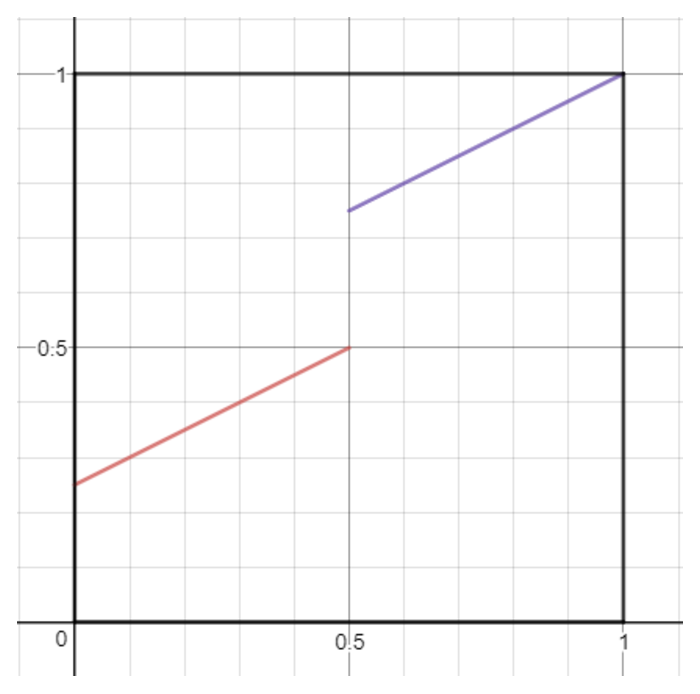
\includegraphics[width=0.2\textwidth]{f.eps}
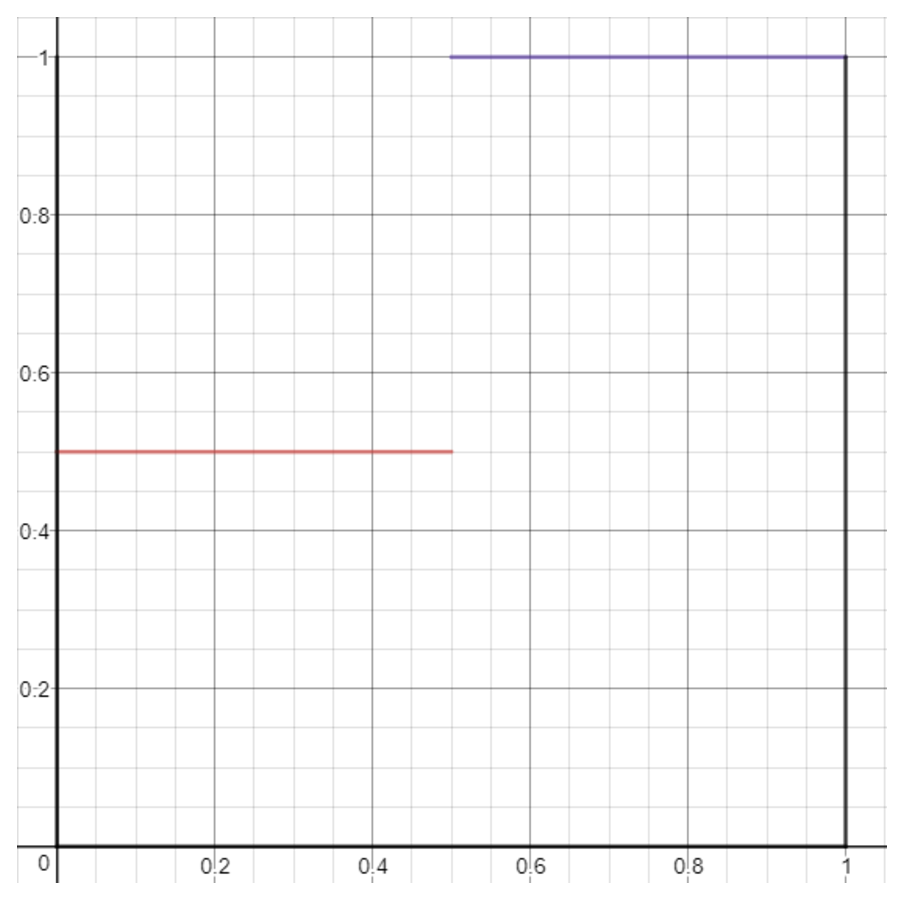
\includegraphics[width=0.2\textwidth]{fw.eps}
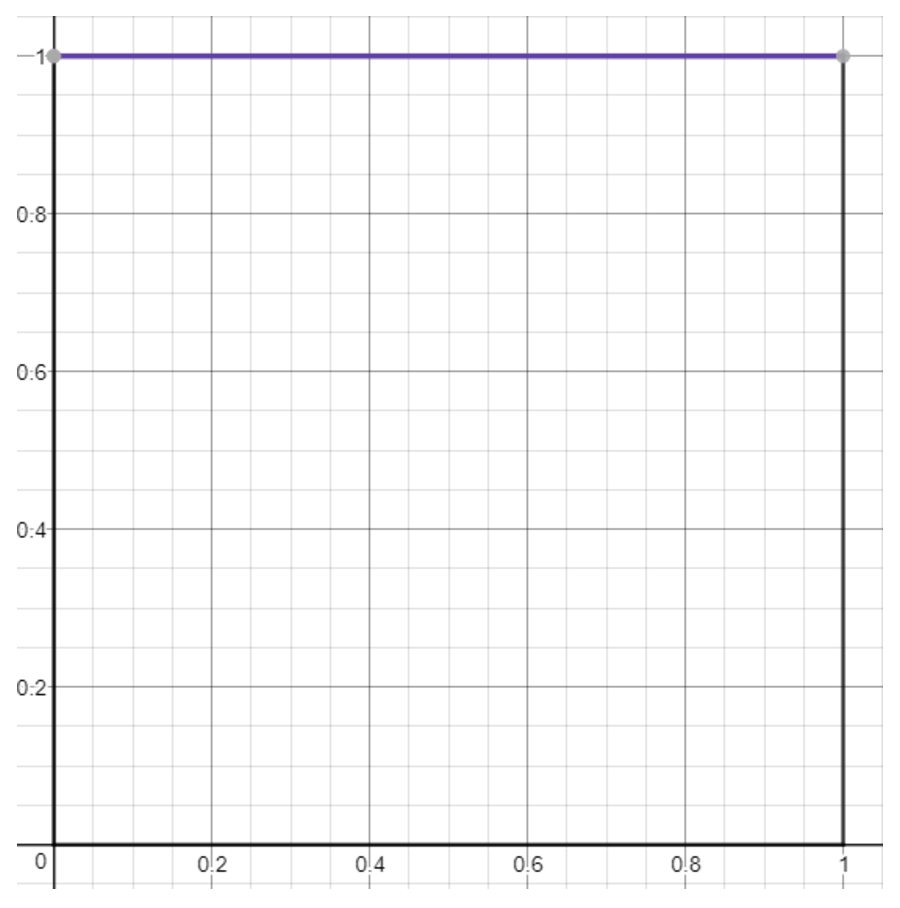
\includegraphics[width=0.2\textwidth]{fww.eps}


\end{exmp}

\begin{exmp}

Пусть $\alpha$ --- ординал. Как определеить $f^{\alpha}$, то есть композицию $f$ с собой $\alpha$ раз? В этом поможет трансфинитная рекурсия.

Согласно принципу трансфинитной индукции достаточно определить, $f^0$ и $\forall \beta < \alpha$ из определения $f^{\gamma}$ вывести определение $f^{\beta}$. Тогда будет определено $f^{\alpha}$.

Пусть $f^0 = id$. Пусть $\alpha$ --- ординал, и $\beta < \alpha$ Тогда
$$f^{\beta}(x) = 
\begin{cases}
f(f^{\beta_1}(x))  & \beta - \textrm{непредельный} \\
f(\lim_{\gamma \rightarrow \beta, \ \gamma<\beta}f^{\gamma}(x)) & \beta - \textrm{предельный, и существует предел}\\
\end{cases}$$
Если для некоторого $x$ предел не существует, то $x$ изымается из области определения, и функция становится частичной.
Пример $f(x) = 1 - x$ 

Если $n$ --- конечный ординал, то 
$$ f^n(x) = \begin{cases}
f(x) = 1 - x & 2|x \\
x & \textrm{иначе} \\
\end{cases}$$
Найдём $f^{\omega}(x)$. В самом деле 
$$ f^n(x) = 
\begin{cases}
1/2 & x = 1/2 \\
\textrm{не определена} & \textrm{иначе}
\end{cases}$$
\end{exmp}

\begin{definition}
Пусть $\alpha$ --- ординал, $f\colon [0,\ 1] \longrightarrow [0,\ 1]$. Точка $x$ называется точкой периода $\alpha$, если $x=f^{\alpha}(x)$, но все точки $f^{\beta}(x)$ разные для всех $\beta < \alpha$. 
 \end{definition}
 
\begin{theorem}{Теорема Шарковского.}

 На $\mathbb{N}$ можно ввести такой порядок $<_{Ш}$, что если  $f : [0,\ 1] \longrightarrow [0,\ 1]$ --- непрерывна и имеет точку периода $n\in\mathbb{N} $, то $f$ имеет также точку всех таких периодов $m\in\mathbb{N}$, что $n<_{Ш} m$
 \end{theorem}
\begin{exmp}
$3 < 5 < 7 < \dots < 2*3 < 2*5 < 2*7 < \dots < 2^2*3 < 2^2*5 < \dots < 2^n*3 < 2^n*5 < \dots < 2^k < 2^{k-1} < \dots < 2 < 1$
\end{exmp}

Обозначим порядковый тип $(\dots < -n < -n + 1 < \dots < -3 < -2 < -1) = \omega^*$. Тогда $\mathbb{N}$ имеет тип $\omega\cdot\omega + \omega^*$.

\subsection{Утверждения, эквивалентные аксиоме выбора}

\begin{definition}
\textbf{Цепью} в упорядоченном множестве называется его подмножество, все элементы которого сравнимы между собой (то есть \textbf{цепь} --- линейно упорядоченное подмножество).
\end{definition}




\begin{theorem}{(Теорема Цермело)}

Каждое множество можно вполне упорядочить.
\end{theorem}

\begin{theorem}{(Теорема Хаусдорфа о цепях)}

В каждом упорядоченном множестве каждая цепь содержится в некоторой максимальной цепи.
\end{theorem}

\begin{theorem}{(Лемма Цорна)}

Если в упорядоченном множестве для каждой цепи имеется верхняя грань, то оно содержит максимальный элемент.
\end{theorem}

\begin{theorem}
Теорема Цермело, теорема Хаусдорфа о цепях и лемма Цорна эквивалентны аксиоме выбора.
\end{theorem}



\section{Кризис наивной теории множеств: парадоксы}

\subsection{Парадоксы}

Парадоксы возникают как следствие неаккуратного обращения с коллективизирующим свойством, то есть не для каждой логической формулы $P$ запись $\{x: P(x)=1\}$ задаёт множество.
\begin{enumerate}
    \item \textbf{Парадокс Кантора}
    $V = \{X: X $ --- множество$\}$ --- класс всех множеств.
    Если считать, что $V$ --- множество, то у него есть множество всех подмножеств $2^V = \{X: X\subset V\}$ Но $2^V \in V$. Более того: $2^V \subset V$, так как $\forall x\in 2^V :\ x\in V$.
    В чём парадокс? С одной стороны, из $2^v \subset V$ следует $|2^V| \leqslant |V|$. С другой стороны, по теореме Кантора $|V| < |2^V|$.
    \item \textbf{Парадокс Рассела}
    $R = \{x: x$ --- множество $ x\notin x\}$. Тогда $R\in R \Longleftrightarrow R\notin R$, что невозможно, поскольку утверждения $R\in R$ и $R\notin R$ являются отрицаниями друг друга.
    \item \textbf{\href{https://en.wikipedia.org/wiki/Burali-Forti_paradox}{Парадокс Буралли-Форти}} $B = \{x: x$ --- ординал $\}$. Противоречие основано на том, что, с одной стороны, для каждого ординала $\alpha$ существует следующий за ним ординал $\alpha+1$ и $\alpha < \alpha+1$, с другой стороны, отправляясь от $B$, можно построить такой ординал $\beta$, что будет $\beta+1<\beta$.
    
\end{enumerate}

Почему парадокс --- это плохо для математики? Потому что в математике с парадоксами сами понятия истинности и ложности теряют смысл. Должно быть: из истины следует истина. Но получится: из истины (при добавлении парадокса) следует ложь. 
\begin{exmp}
Как извлечь из истины ложь? Пусть 2*2 = 4 --- истина. Положим $R = \{x: x$ -- множество, $x\notin x\}$. Тогда $R\in R \Longleftrightarrow R\notin R$, но $R\in R \Longleftrightarrow R\notin R$ --- ложно.
\end{exmp}

Ответ математического сообщества на открытие парадоксов:

\textbf{Открытие аксиоматической теории множеств}
    
    Аксиомы ограничивают математика при построении построении новых множест из уже имеющихся таким образом, что приводящии к парадоксам "множества"\ $V,\ R,\ B$ и другие построить нельзя, то есть $V,\ R,\ B$ существуют как классы, а не как множества. К классам не применимы понятия мощность и другие, поэтому парадоксов при обращении с настоящими множествами, построенными на аксиомах теории множеств, не возникает, все парадоксы остались с классами (как угодно построенными семействами объектов, которые использовать в строгих доказательствах запретили).

\subsection{Аксиомы теории множеств (аксиомы Цермело-Френкеля)}\label{ZFC}
\begin{remark}
Теория множеств говорит только о множествах, то есть все объекты --- множества. В частности, элементами множеств могут быть \textbf{только} множества! Кроме множеств ничего нет.
\end{remark}

    \begin{axiom}{Объёмности, равенства}
\begin{enumerate}
        \item  Объёмности. Множества $A$ и $B$ равны $\Longleftrightarrow (x\in A \Longleftrightarrow x\in B)$
        \item Равенства. Равные множества $x$ и $y$ являются элементами одних и тех же множеств, то есть $x=y \Longleftrightarrow (\{z: x\in z\} = \{w: y\in w\})$
\end{enumerate}
    \end{axiom}
    \begin{axiom}{Аксиома пары.} Для любых множеств $x$ и $y\ \exists \{x,\ y\}$ --- множество, единственными элементами которого являются $x$ и $y$. В частности, если $x=y$ $\exists \{x,\ y\} = \{x,\ x\} = \{y,\ y\}=\{y\}=\{x\}$.
    \end{axiom}
    \begin{axiom}{Схема аксиома выделения.} $\forall$ свойства $\varphi(x)$ и множества $X\ \exists Y$ --- множество, $Y = \{x\in X: \varphi(x)\}$ содержащее те и только те точки $x\in X$, для которых верно $\varphi(x)$.
    \end{axiom}
    \begin{remark}
    $\varphi$ --- предикат, так как в выражение $\varphi(x)$ переменная $x$ пробегает указанное множество $X$.
    \end{remark}
    \begin{remark}
    Схема аксиома позволяет определить пересечение множеств: $A\cap B = \{x\in A: x\in B\}$
    \end{remark}
    \begin{axiom}{Аксиома объединения.} Если $X$ --- множество, то $\exists \bigcup X = \{x: \exists y\in X:\ x\in y\}$
    \end{axiom} 
    \begin{remark}
    Из аксиомы пары и аксиомы объединения можно определить объединение двух множеств. Если $A$ и $B$ --- множества, то по аксиоме пары $\{A,\ B\}$ --- множество, и по аксиоме объединения $\exists \bigcup \{A,\ B\} = A\cup B$
    \end{remark}
    \begin{axiom}{Аксиома степени.} $\forall X\ \exists\mathcal{P}(X)$ --- множество всех подмножеств множества $X$
    \end{axiom} 
    \begin{definition}
        Множество $S$ называется \textbf{индуктивным}, если выполняются два условия:
        \\1) $\varnothing\in S$
        \\2) $x\in S \Longrightarrow (x\cup\{x\})\in S$
    \end{definition}
    \begin{axiom}{ Аксиома бесконечности, она же аксиома индуктивного множества.} Существует индуктивное множество (хотя бы одно).
    \end{axiom}
    
    \begin{exmp}
    $\varnothing\in S \Longrightarrow \varnothing\cup\{\varnothing\} = \{\varnothing\}\in S$
    
    $\{\varnothing\}\in S \Longrightarrow \{\varnothing\}\cup \{\{\varnothing\}\} = \{\varnothing,\ \{\varnothing\}\}\in S$
    
    $\{\varnothing,\ \{\varnothing\}\}\in S \Longrightarrow \{\ \ \varnothing,\ \ \{\varnothing\},\ \ \{\{\varnothing, \{\varnothing\}\}\}\ \ \}\in S $
    \end{exmp}
    
    \begin{axiom}{Аксиома регулярности.} Если $x\neq \varnothing$, то $\exists a\in x:\ \forall y\in x\ \textrm{верно}\ y\notin a$
    \end{axiom} 
    
    \begin{corollary}\label{x_notin_x}
    Никакое множество не является своим элементом, то есть $\forall x\ \textrm{верно}\ x\notin x$
    \begin{proof}
    По аксиоме пары существует множество $\{x, x\}$, которое равно $\{x\}$ по аксиоме объёмности, так как $\{x, x\}$ и $\{x\}$ имеют одни и те же элементы. Применим к $x$ аксиому регулярности. Тогда в $\{x\}$ должен найтись такой $a$, что $y\notin a$ для всех $y\in\{x\}$. Но в \{x\} только один элемент - это $x$, поэтому $a=y=x$, то есть $x\notin x$
    \end{proof}
    \end{corollary}
    
    \begin{axiom}{Схема аксиом подстановки.} Пусть $\varphi(x,\ y)$ при любых $x,\ y$ истинно или ложно. Пусть $\forall x\ \exists$ не более одного такого $y$, что верно $\varphi(x,\ y)$. Тогда $\forall A\ \exists B=\{y: \exists x\in A\ \textrm{что верно}\ \varphi(x,\ y)\}$.
    \end{axiom}
    \begin{axiom}{Аксиома выбора.} Если $S$ --- непустое множество непустых множеств, то $\exists f$ --- функция $f\colon S\to \cup S$ такая ($\cup S$ существует по аксиоме объединения), что $f(x)\in x$ для всех $x\in S$
    \end{axiom}

\begin{remark}
Аксиомы 1 -- 8 вместе обозначаются ZF (Цермело-Френкеля), а 1--9 вместе обозначаются ZFC (Zermelo-Fraenkel-Choice).
\end{remark}

\begin{theorem}\label{per_ind_ind}
Пересечение любого непустого множества индуктивных множеств является индуктивным множеством.
\begin{proof}
Пусть $A\neq\varnothing,\ \forall x\in A\ x$ --- индуктивное. Пусть $B = \bigcap_{x\in A}x$. Тогда:
\\1) $\forall x\in A : \varnothing\in x$. Значит, $\varnothing\in B$.
\\2) Пусть $y\in B$. Тогда $y\in x\ \forall x\in A$. Но $x$ --- индуктивно, поэтому $y\cup \{y\}\in x$. Поэтому ($B$ --- пересечение всех $x\in A$)$y\cup \{y\}\in B$.
\end{proof}
\end{theorem}
\begin{corollary}\label{coroll_min}
Cуществует и единственно такое индуктивное множество $N$, что $N\subset X$ --- для любого индуктивного $X$. (Неформально говоря, существует наименьшее по включению индуктивное множество $N$).
\begin{proof}

\textit{Существование.} По аксиоме бесконечности существует индуктивное множество $S$. По аксиоме степени существует $\mathcal{P}(S)$. По аксиоме выделения $\exists \{x\in\mathcal{P}(S): x \textrm{--- индуктивно}\} = A$. Так как $S\in \mathcal{P}(S)$ и $S$ --- индуктивное, верно, что $A\neq \varnothing$. Пусть $B = \bigcap_{x\in A} x$. По только что доказанной теореме о пересечении индуктивных множеств $B$ --- индуктивное. Пусть теперь $G$ --- любое индуктивное множество. Тогда $G\cap S$ --- индуктивное по той же теореме. Но $G\cap S \subset S$, поэтому $(G\cap S)\in \mathcal{P}(S)$.

$
\left.
\begin{array}{c}
     G\cap S \textrm{--- индуктивное} \\
     G\cap S\in \mathcal{P}(S)
\end{array}
\right\}
\Longrightarrow G\cap S\in A
$

Тогда в пересечении $\bigcap_{x\in A} x=B$ какой-то $x$ равен $G\cap S$, поэтому $B\subset G\cap S$. Получаем, что $B\subset (G\cap S)\subset G$, то есть $B\subset G$ для любого индуктивного множества $G$.

\textit{Единственность.} Пусть $N_1$ и $N_2$ ---  два таких множестваю Но оба они индуктивные и лежат в каждом индуктивном, поэтому $N_1\subset N_2,\ N_2\subset N_1$. Отсюда по аксиоме объёмности следует, что $N_1 = N_2$.
\end{proof}
\end{corollary}


\section{Натуральные числа и их свойства}
\begin{remark}
Все свойства натуральных чисел (и всех объектов, построенных только из натуральных чисел) полностью могут быть выведены из:
\\1) Двух неопределяемых понятий: первое натуральное число (обозначаемое 0 или 1 в зависимости от договорённости), следующее натуральное число (имеется в виду следующее за данным натуральным числом).
\\2) Пяти постулатов (аксиом) Пеано.
\end{remark}

\subsection{Аксиомы Пеано}

Обозначим множество всех натуральных чисел буквой $N$, первое натуральное число $0$, следующее за $x$ натуральное число символом $x'$. 

Тогда аксиомы Пеано записываются так: 

\begin{axiom}
$0\in N$
\end{axiom}

\begin{axiom}
$\forall x\in N\ \exists ! x'\in N$. Единственность означает, что из $x=y$ следует $x'=y'$.
\end{axiom}

\begin{axiom}
$\forall x\in N: x'\neq 0$
\end{axiom}

\begin{axiom}
$(x' = y') \Longrightarrow (x=y)$
\end{axiom}

\begin{axiom}
(аксиома индукции) Пусть $A\subset N$ и верно следующее:
\\1)$0\in A$
\\2)$(x\in A)\Longrightarrow (x'\in A)$.

Тогда $A=N$
\end{axiom}


\subsection{Определение натуральных чисел и вывод аксиом Пеано из ZF}

\begin{definition}
Положим: 

$N = $ наименьшее по включению индуктивное множество, его существование и единственность были доказаны выше; 

$0 = \varnothing$; 

$x'=x\cup\{x\}$.
\end{definition}

Докажем постулаты (аксиомы) Пеано, опираясь на эти опеределения для $N, 0, x'$ и аксиомы ZF.
\begin{proof}{}\label{proof_nat}

1) По определению индуктивного множества (часть 1) $\varnothing\in N$, но $0=\varnothing$, значит $0\in N$.

2) По определению индуктивного множества (часть 2) из $x\in N$ следует $x\cup\{x\}=x'\in N$ по аксиоме объёмности  множество $x\cup \{x\}$ строится по $x$ однозначно, то есть если $x=y$, то $x' = x\cup \{x\} = y\cup \{y\} = y'$.

3) Если $y = x'$ для некоторого $x$, то $y = x\cup \{x\}\neq \varnothing$, так как $x\in y$. Но $0=\varnothing$, поэтому $x' = y \neq \varnothing = 0$, то есть $x'\neq 0$.

4) От противного. Пусть $x' = y'$, но $x\neq y$. Рассмотрим цепочку импликаций 
$x' = y' \Longleftrightarrow x\cup \{x\} = y\cup \{y\} \Longrightarrow 
\begin{cases}
     x\subset y\cup \{y\}  \\
     y\subset x\cup \{x\} 
\end{cases} \Longrightarrow
\begin{cases}
     x\in y\cup \{y\}  \longrightarrow 
     \begin{cases}
         x\in \{y\} \textrm{ --- невозможно, так как } x\neq y  \\
         x\in y
     \end{cases}\\
     y\in x\cup \{x\}  \longrightarrow
     \begin{cases}
         y\in \{x\} \textrm{ --- невозможно, так как } x\neq y  \\
         y\in x
     \end{cases}
\end{cases}
$
Получили, что верны оба утверждения: $x\in y$ и $y\in x$, так как остальные возможности уже исключены в силу того, что $x\neq y$. Это порождает бесконечную вправо и влево цепочку принадлежности $\dots \in x\in y\in x\in y\in x\in \dots$. Аксиома регулярности позволяет показать, что невозможна (см. следствие \ref{x_notin_x}) не только цепочка $\dots \in x\in x\in x\in x\in x\in \dots$, но и только что возникшая цепочка из $x$ и $y$.

В самом деле, по аксиоме пары существует множество $\{x,\ y\}$, элементы которого различны, так как $x\neq y$. Применим к $\{x,\ y\}$ аксиому регулярности: $\exists a\in \{x,\ y\} : \begin{cases}
     x\notin a\\
     y\notin a
\end{cases}$ Но в $\{x,\ y\}$ два элемента, поэтому $a=x$ или $a=y$. 

Если $a=x$, то $\begin{cases}
     x\notin x \textrm{ --- невозможно по следствию \ref{x_notin_x}}\\
     y\notin x \textrm{ --- противоречит } y\in x
\end{cases}$.

Если $a=y$, то $\begin{cases}
     y\notin y \textrm{ --- невозможно по следствию \ref{x_notin_x}}\\
     x\notin y \textrm{ --- противоречит } x\in y
\end{cases}$.

Таким образом, стартовав с $x' = y'$ и $x\neq y$, мы пришли к тому, что $x\in y\in x$, что невозможно. Постулат 4 доказан.

5) если $0\in A$ и $x\in A \Longrightarrow x'\in A$, то $A$ --- индуктивно ($0=\varnothing,\ x'= x\cup \{x\}$
Но $N$ --- наименьшее по вложению индуктивное множество, поэтому $N\subset A$. Но по условию $A\subset N$, значит $A=N$ по аксиоме объёмности.
\end{proof}

\newpage
\section{Список вопросов к экзамену}
\begin{enumerate}
\item  Сформулируйте определение высказывания. Приведите примеры фраз, являющихся и не являющихся высказываниями.

\item  Сформулируйте определение предиката. Приведите примеры фраз, являющихся и не являющихся предикатами.

\item Что такое логические константы 0 и 1? Приведите примеры высказываний, равных 0; равных 1. Может ли высказывание быть одновременно равно 0 и 1, почему (когда)?

\item  Что такое кванторы? Какие два квантора обсуждались в курсе? Приведите примеры их использования: сформулируйте несколько предикатов и сделайте из них константы с помощью кванторов. 

\item  Приведите примеры логических функций с их таблицами истинности.

\item Что такое множество (дайте неформальное описание)? Назовите подходы к теории множеств и скажите, в чём они состоят. Какие существуют способы задания множеств?

\item Дайте неформальное описание функции в широком и в узком смысле.

\item  Что называется характеристической функцией множества? Какие значения она может принимать?

\item Какие существуют операции над множествами? Приведите их определения и и задание через характеристические функции.

\item Нарисуйте круги Эйлера для основных операций над множествами. 


\item  Сколько существует подмножеств у множества из $n$ элементов? Сформулируйте и двумя способами  докажите теорему ~\ref{teorem_2A} о количестве подмножеств у конечного множества (сложность 2)

\item Сформулируйте формулу включений-исключений для случая двух и трёх множеств.

\item Сформулируйте определение неупорядоченной пары

\item Сформулируйте определение упорядоченной пары

\item Что называют декартовым произведением множества $A$ на множество $B$? 

\item Что называют бинарным отношением  на множестве?

\item Какое отношение на множестве называется рефлексивным, а какое антирефлексивным? В чём состоит геометрический смысл рефлексивности и антерефлексивности отношения на множестве?
                                                          
\item Какое отношение на множестве называется симметричным, а какое антисимметричным?

\item Какое отношение на множестве называется транзитивным?

\item Какое отношение называют связным (в другой терминологии --- полным)?

\item Какое отношение называют отношением предпочтения? Объясните, как отношение предпочтения задаётся с помощью функции полезности. Каждое ли отношение предпочтения можно задать с помощью функции полезности?

\item  Что называют отношением эквивалентности на множестве? Что называют классом эквивалентности элемента по отношению эквивалентности? Что называют факторизацией?

\item Что называют классом эквивалентности элемента по отношению эквивалентности?  Докажите, что классы эквивалентности либо не пересекаются, либо совпадают (Теорема ~\ref{eq_t}).(сложность 1)

\item Что называют разбиением множества? Докажите, что каждое отношение эквивалентности на множестве однозначно задаёт разбиение множества. Сформулируйте и докажите обратное утверждение ~\ref{razb}.(сложность 3)

\item  Что называют отношением порядка? Что называют отношением строгого порядка?

\item  Что называют верхней гранью упорядоченного множества? Что называют точной верхней гранью упорядоченного множества?

\item  Что называют нижней гранью упорядоченного множества? Что называют точной нижней гранью упорядоченного множества?

\item  Что называют упорядоченной суммой упорядоченных множеств? Коммутативна ли сумма упорядоченных множеств?

\item  Что называют упорядоченным произведением упорядоченных множеств? 

\item Что называют функцией? Что называют областью определения, множеством принимаемых значений? 

\item  Какая функция называется инъективной?

\item  Какая функция называется сюръективной?

\item  Какая функция называется биективной?

\item  Какая функция называется обратимой?

\item Что называется функцией? Какая функция называется биективной? Какая функция называется обратимой? Докажите, что функция биективна тогда и только тогда, когда она обратима (Теорема ~\ref{biek_obr}).(сложность 1)

\item Какая функция называется биективной? Докажите, что обратная к биекции функция --- тоже биекция (Следствие ~\ref{corollary_biek_biek}).(сложность 1)

\item  Какая функция называется биективной? Докажите, что композиция биекций --- биекция (Утверждение ~\ref{biek_comp}).(сложность 1)

\item  В каком случае говорят, что множество $B$ проиндексировано с помощью множества индексов $A$? Приведите примеры.

\item Объясните, как развести пересекающиеся множества.

\item Сформулируйте аксиому выбора. 

\item Сформулируйте аксиому выбора. Сформулируйте определение декартова произведения семейства множеств $\{X_\alpha: \alpha\in A\}$, проиндексированных некоторым множеством $A$, т.е. произведение всех $A_\alpha$ по $\alpha\in A$.  Докажите, что аксиома выбора равносильна тому, что декартово произведение непустого множества непустых дизъюнктных множеств непусто (Утверждение ~\ref{choice_th}). (сложность 2)

\item Сформулируйте и докажите принцип Дирихле в двух частях (Утверждение ~\ref{dir}). (сложность 2)

\item Пусть функция отображает конечное множество в себя. Пусть известно, что если она обладает любым из трёх свойств --- инъективность, сюръективность, биективность; что можно сказать о том, обладает ли она двумя другими из этих свойств? Докажите соответствующую теорему. (Утверждение~\ref{A_to_A}). (сложность 2) 

\item  Сформулируйте три определения бесконечного множества. Докажите их эквивалентность (Утверждение~\ref{infinity}).(сложность 3)

\item  Сформулируйте три определения конечного множества. Докажите их эквивалентность со ссылкой на аналогичный факт про бесконечные множества.(сложность 1)

\item  Какое множество называется счётным? Не более, чем счётным?

\item  Когда говорят, что два множества равномощны? Что называют мощностью (кардинальным числом, кардиналом) множества?

\item  Когда говорят, что мощность $B$ не больше мощности $A$? Сформулируйте три определения и докажите их эквивалентность (Утверждение~\ref{geqmn}).(сложность 2)

\item  Когда говорят, что мощность $B$ строго больше мощности $A$? 

\item  Пусть $A$ и $B$ --- множества. Что обозначается символом $A^B$? Символом $P(A)$? Докажите теорему, устанавливающую соотношение между мощностями $|P(A)|$, $|\{0,1\}^A|$, $|\{x,y\}^A|$, где $x\neq y$ --- любые различные объекты (Утверждение~\ref{01A}).(сложность 2)

\item  Что называют последовательностью точек множества?

\item  Сформулируйте и докажите теорему~\ref{Kantor}  Кантора о соотношении между мощностью множества и мощностью множества всех его подмножеств.(сложность 3)

\item  Сформулируйте <<лемму о двух теоретико-множественных милиционерах>>. На сколько шагов в курсе разбито доказательство этой леммы? Что в доказательстве было названо <<хорошим множеством>>?

\item  Сформулируйте и докажите <<лемму о двух теоретико-множественных милиционерах>>.  (Лемма~\ref{police}). (сложность 3)

\item  Сформулируйте и докажите теорему~\ref{KSHB} Кантора-Шрёдера-Бернштейна.(сложность 1)

\item  Какая функция называется монотонной?

\item Какие множества называются изоморфными в смысле порядка? Что называют порядковым типом множества?

\item  Когда говорят, что одно множество плотно в другом в смысле порядка? Приведите примеры.

\item  Какое множество называют вполне упорядоченным?

\item  Что назыают ординалами (ординальными числами)? 

\item Что называют цепью?

\item  Сформулируйте правило~\ref{sum_ord} сложения и умножения ординалов. Сформулируйте утверждения о том, что эти правила корректны. 

\item Докажите корректность правила~\ref{sum_ord} сложения ординалов.(сложность 3) 

\item  Что называют трансфинитами (трансфинитными числами)?

\item Сформулируйте три вида математической индукции. Равносильны ли они?

\item Что называют начальным отрезком в линейно упорядоченном множестве?

\item Сформулируйте теорему~\ref{sravn_ord} о сравнении ординалов в терминах начальных отрезков.

\item Пусть $\alpha$ --- ординал. Определите ординал $\alpha + 1$. Объясните, как вводится стандартное отношение порядка на любом множестве ординалов. Линейный ли это порядок? Докажите теорему, утверждающую, какой из ординалов $\alpha$ и $\alpha + 1$ больше в смысле этого отношения порядка. (Теорема~\ref{coroll_alp_alp1}). (сложность 1)

\item Что называют нулевым ординалом?

\item Что называют стандартным представлением ординала? Сформулируйте теорему~\ref{stand_ord} о стандартном представлении ординала.

\item Сформулируйте и докажите теорему о сравнении множеств по мощности (Теорема~\ref{srav_po_mosh}).(сложность 1)

\item Какой ординал называют предельным; непредельным?

\item Сформулируйте и докажите принцип трансфинитной индукции (Теорема~\ref{transfinit}).(сложность 2)

\item Объясните, что такое трансфинитная рекурсия.

\item Сформулируйте определение того, что $f_0 = \lim_{\beta \rightarrow\beta_0,\ \beta < \beta_0}f(\beta)$, где $f_0$ --- число, $\beta_0$ --- предельный ординал, а $f\colon \beta_0\to\mathbb{R}$.

\item Как определить $f^{\alpha}$, где $\alpha$ --- ординал, а функция $f$ отображает отрезок $[a,b]$ в себя?

\item Приведите пример такой функции $f\colon [0,1]\to [0,1]$, что функции\\ $f, f^2, f^3, \dots, f^\omega, f^{\omega+1}, f^{\omega+2},\dots, f^{\omega+\omega}$ все различны.

\item Что называют точкой периода $\alpha$ функции $f: [0,\ 1] \longrightarrow [0,\ 1]$, где $\alpha$ --- ординал?

\item Сформулируйте теорему Цермело.

\item Сформулируйте теорему Хаусдорфа о цепях.

\item Сформулируйте лемму Цорна.

\item Сформулируйте теорему о непустоте декартова произведения.

\item Сформулируйте утверждения, эквивалентные аксиоме выбора (5 шт. вместе с самой аксиомой выбора).

\item В чём состоит парадокс Кантора в наивной теории множеств?

\item В чём состоит парадокс Рассела в наивной теории множеств?

\item На чём основан парадокс Буралли-Форти в наивной теории множеств?

\item Сформулируйте аксиомы объёмности и равенства в системе аксиом ZF.

\item Сформулируйте аксиому пары в системе аксиом ZF.

\item Сформулируйте схему аксиом выделения в системе аксиом ZF.

\item Сформулируйте аксиому объединения в системе аксиом ZF.

\item Сформулируйте аксиому степени в системе аксиом ZF.

\item  Какое множество называется индуктивным? Сформулируйте аксиому индуктивного множества (она же аксиома бесконечности).

\item Сформулируйте аксиому регулярности в системе аксиом ZF. Докажите, что никакое можество не является своим элементом (Следствие~\ref{x_notin_x}).(сложность 1)

\item Сформулируйте схему аксиом подстановки в системе аксиом ZF.

\item Сформулируйте аксиому выбора (в формулировке ZFC ~\ref{ZFC}).

\item Перечислите названия всех аксиом ZF. Объясните, в чём состоит отличие ZFC от ZF.

\item Докажите, что пересечение любого непустого множества индуктивных множеств является индуктивным множеством(Теорема~\ref{per_ind_ind}).(сложность 2)

\item Докажите, что существует и единственно такое индуктивное множество $N$, что $N\subset X$ --- для любого индуктивного $X$ (Следствие~\ref{coroll_min}). Как связаны $N$ и $\mathbb{N}$? (сложность 3)

\item Какие два неопределяемых понятия задают натуральные числа в аксиоматике Пеано? Сформулируйте аксиомы Пеано. 

\item Докажите, что аксиомы Пеано являются следствием аксиом  ZF (Доказательство~\ref{proof_nat}). (сложность 3) 
\end{enumerate}


\newpage
\section{Задачи к экзамену}


{\bf Тема 1. Записать утверждение с помощью логических функций и кванторов. Обратная задача: прочитать такую запись.}\\


Тема 1. Задача сложности 1.

$p(x)=x$ скачет по болоту

$q(y)=y$ является лягушкой

Записать утверждение <<все лягушки скачут по болоту>>

Прочитать запись <<$\exists y:\overline{q(y)}\wedge p(y)$>>\\

Тема 1. Задача сложности 2.

$p(x)=x$ скачет по болоту

$q(y)=y$ является лягушкой

$w=$идёт дождь

Записать утверждение <<если по болоту скачут не только лягушки, то дождя нет>>

Прочитать запись <<$\exists y:(p(y)\rightarrow w)\rightarrow p(y)$>>\\





{\bf Тема 2. С помощью диаграмм Эйлера или Венна сравнить два множества.}\\

Тема 2. Задача сложности 1. Сравнить $A\cap B$ и $A\setminus(B\setminus(A\cap B))$\\

Тема 2. Задача сложности 2. Сравнить $(A\cup B)\setminus C$ и $(A\setminus C)\Delta (B\setminus(A\cap B))$\\



{\bf Тема 3. Переход от записи множества в виде операций над известными множествами к записи в виде множества всех элементов, для которых выполняется некоторое условие. И обратно.}\\

Тема 3. Задача сложности 1. Представить $(A\cap B)\setminus C $ в виде $\{x:\ \dots\}$\\

Тема 3. Задача сложности 2. Выразить с помощью операций над множествами $A,\ B,\ C$ множество $\{x:\ (x\in A) \vee ((x\notin B) \wedge (x\notin C))\}$\\

{\bf Тема 4. Задача на формулу включений-исключений.}\\

Тема 4. Задача сложности 1. В классе 10 учеников, и каждый любит хотя бы один предмет из списка: физика, математика. Физику любят 5 человек, математику -- 8 человек. Сколько учеников любят одновременно физику и математику?\\

Тема 4. Задача сложности 2. В классе 20 учеников, и каждый любит хотя бы один предмет из списка: литература, биология, история. Литературу любят 10 человек, биологию -- 20, историю -- 13. Одновременно литературу и биологию -- 10, литературу и историю -- 10, историю и биологию -- 10. Сколько учеников любят все три предмета?\\

{\bf Тема 5. Исследовать свойства бинарного отношения.}\\

Тема 5. Задача сложности 1. Отношение $R$ на $\mathbb{N}$ задано так: $xRy\iff$ число $x/y$ является целым числом. Исследовать свойства отношения $R$.\\

Тема 5. Задача сложности 2. Отношение $R$ на $\mathbb{N}\times \mathbb{N}$ задано так: $(x_1,x_2)R(y_1,y_2)\iff$ число $x_1/y_2$ является целым числом. Исследовать свойства отношения $R$.\\



{\bf Тема 6. Исследовать отношение порядка - найти минимальные, максимальные элементы, ответить на другие вопросы.}\\

Тема 6. Задача сложности 1. Пусть $A$ --- множество из четырёх элементов, и $B$ --- множество всех подмножеств множества $A$, состоящих из не более, чем 3 элементов. Отношение $R$ на $B$ задано так: $A_1RA_2\iff(A_1\subset A_2)$. Является ли $R$ отношением порядка, строгого порядка, линейного порядка, частичного порядка? Нарисовать диаграмму Хассе, указать: наибольшие, наименьшие, максимальные, минимальные элементы. Применить к $B$ теорему Хаусдорфа, теорему Цермело, указать результат применения. Применима ли к $B$ лемма Цорна? Если применима, то указать результат применения.\\

Тема 6. Задача сложности 2. Построить бесконечное упорядоченное множество, к которому не применима лемма Цорна и имеющее три максимальных элемента и наименьший элемент.\\

{\bf Тема 7. Исследовать отношение эквивалентности. Описать классы, при возможности --- составить рисунок.}\\

Тема 7. Задача сложности 1. Определим на $\mathbb{R}$ отношение $R$ так: $xRy\iff x^2=y^2$. Проверить, что $R$ является отношением эквивалентности. Найти классы эквивалентности. Указать мощность классов эквивалентности. Указать мощность фактор-множества.\\

Тема 7. Задача сложности 2. Определим на $\mathbb{R}^2$ отношение $R$ так: $(x_1,y_1)R(x_2,y_2)\iff x_1^2+y_1^2=x_2^2+y_2^2$. Проверить, что $R$ является отношением эквивалентности. Найти классы эквивалентности. Указать мощность классов эквивалентности. Указать мощность фактор-множества.\\


{\bf Тема 8. Исследовать функцию на инъектианость, сюръективность, биективность, монотонность. В случае обратимости найти обратную функцию и исследовать её.}\\

Тема 8. Задача сложности 1. Исследовать функцию $f\colon \mathbb{R}\to \mathbb{R}$, $f(x)=x\sin(x)$ на инъектианость, сюръективность, биективность, монотонность (порядок на $\mathbb{R}$ зададим так: $x\leq y\iff (x^3\leq y^3)$). В случае обратимости найти обратную функцию и исследовать её.\\

Тема 8. Задача сложности 2. Исследовать функцию $f\colon \mathbb{R}^2\to \mathbb{R}^2$, $f(x,y)=(y,x^5)$ на инъектианость, сюръективность, биективность, монотонность (порядок на $\mathbb{R}^2$ зададим так: $(x_1,y_1)\leq (x_2,y_2)\iff (x_1\leq x_2)\wedge (y_1\leq y_2)$). В случае обратимости найти обратную и исследовать её.\\



{\bf Тема 9. Сравнить мощности двух множеств или найти мощность множества.}\\

Тема 9. Задача сложности 1. Найти мощность множества $\mathbb{N}\times \mathbb{N}\times \mathbb{N}$.\\

Тема 9. Задача сложности 2. Найти мощность множества $\mathbb{N}^\mathbb{N}$.\\


{\bf Тема 10. Сложить и умножить ординалы.}\\

Тема 10. Задача сложности 1. Пусть $\alpha=\omega, \beta=3$. Привести примеры множеств, упорядоченных по типам $\alpha$ и $\beta$. Построить множества, упорядоченные по типам $\alpha+\beta, \beta+\alpha, \alpha\cdot\beta, \beta\cdot\alpha$, предложить наиболее простые записи для их порядковых типов.\\

Тема 10. Задача сложности 2. Пусть $\alpha=\omega\cdot 2, \beta=3\cdot \omega$. Привести примеры множеств, упорядоченных по типам $\alpha$ и $\beta$. Построить множества, упорядоченные по типам $\alpha+\beta, \beta+\alpha, \alpha\cdot\beta, \beta\cdot\alpha$, предложить наиболее простые записи для их порядковых типов.\\


{\bf Тема 11. Определить, по какому типу упорядоченно множество. Обратная задача: построить множество, упорядоченное по данному типу.}\\

Тема 11. Задача сложности 1. Обозначим порядковый тип множества всех отрицательных целых чисел с обычным порядком символом $\omega^*$. Привести пример множества, упорядоченного по типу $\omega+\omega^*$. Выразить через конечные ординалы, $\omega, \omega^*$ порядковый тип подмножества всех натуральных чисел, состоящего из 1 и всех натуральных степеней чисел 2,3,5,  упорядоченного так: $$2<4<8<16<...<3<9<27<81<...<1<...<125<25<5$$

Тема 11. Задача сложности 2. Обозначим порядковый тип множества всех отрицательных целых чисел с обычным порядком символом $\omega^*$. Привести пример множества, упорядоченного по типу $\omega+(\omega^*\cdot \omega^*)$. Выразить через конечные ординалы, $\omega, \omega^*$ порядковый тип множества $A=\{m+\frac{1}{n+1} | m\in\mathbb{Z}, n\in\mathbb{N}\}$, где $\mathbb{N}=1,2,3,\dots$, а множество $A$ наследует порядок с обычного порядка на вещественной оси.\\  


{\bf Тема 12. Доказать равенство или неравенство с помощью метода математической индукции.}\\

Тема 12. Задача сложности 1. Начиная с какого $n_0\in\mathbb{N}$ начинает выполняться неравенство $2^n\geq n^2$? Докажите это неравенство по индукции, приняв $n_0$ за базу индукции.\\

Тема 12. Задача сложности 2. Начиная с какого $n_0\in\mathbb{N}$ начинает выполняться равенство $1^2+2^2+\cdots+n^2=\frac{1}{6}n(n+1)(2n+1)$? Докажите это равенство по индукции, приняв $n_0$ за базу индукции.


\end{document}